
Purely hadronic events originating from QCD interactions in proton-proton collisions account for the vast majority of events observed at the LHC. Not surprisingly, these events are a major background to new physics signals that may manifest in the hadronic channel, particularly in regions of low $\met$. Several features of multi-jet QCD events are poorly modeled, including the production cross section, jet multiplicity, and relationships between the directions of jets. This motivates the development of data-driven approaches to QCD estimation. Generally, one takes advantage of the particularly well-modeled aspects of event simulation, but relies on the real data to model as many features as possible. As with any data-driven approach, the method must be robust against possible signal contamination that may enter into control regions. 

\subsection{The origin of $\met$ in QCD events}
In order to estimate the QCD background contribution in signal regions with large $\met$, it is relevant to note that the only stable particles in the standard model that are invisible to the CMS detector are neutrinos. Apart from rare final states containing heavy-flavor jets,  QCD events are free of neutrinos, and therefore exhibit little or no $\met$ at the parton level.  For this reason, the $\met$ typically serves as an excellent discriminating variable between the large QCD background and events with significant $\met$, such as models of $R$-parity conserving supersymmetry. However, QCD events {\it only} exhibit zero $\met$ at the parton level $(\met)_{\rm part}$. The final-state particles are detected by a tracker and calorimeters with finite momentum and energy resolution. Mis-measurements of the jet momenta propagate into the measured missing transverse energy, which can result in the measurement of large missing transverse energy, $(\met)_{\rm meas}$, and so QCD events can occupy a similar kinematic region as events predicted by models of new physics.  These statements can be summarized as follows:
\begin{align}
%\begin{split}
(\vec{E}_{ T}^{\rm miss})_{\rm part} &\equiv -\sum_{i=1}^{n}(\vec{p}_{T})_{i,\rm part\ }=0\\
(\vec{E}_{ T}^{\rm miss})_{\rm meas} &\equiv -\sum_{i=1}^{n}(\vec{p}_{T})_{i,\rm meas\ \ \ }\neq 0,
%\end{split}
\label{eq:metTrue}
\end{align}
where $i$ is the particle index and $n$ is the number of particles in the event.

\subsection{Model assumptions and likelihood} 
In general, the magnitudes of the four-vectors of jets at the parton and reconstruction levels differ. However, assuming their directions are identical, the following expression holds for the collection of $n$ jets of a given event,
\begin{equation}
\vec{J}_{\rm meas} = \hat{C} \vec{J}_{\rm part},
\end{equation}
where $\vec{J}_{\rm meas}$ and $\vec{J}_{\rm part}$ are $n\times 1$ vectors of the reconstructed jet four-vectors and the parton-level jet four-vectors, and $\hat{C}$ is diagonal $n\times n$ matrix whose elements are the jet energy scale factors $(c_1,c_2,...,c_n)$. The likelihood for a scale factor $c_i\equiv p^{\mu}_{i,\rm meas}/p^{\mu}_{i,\rm part}$, given by
\begin{equation}
L_{i}\equiv{\rm P}(p^{\mu}_{i,\rm meas}|\ p^{\mu}_{i,\rm part})={\rm P}(c_i\ |\ p^{\mu}_{i,\rm part}),
\label{eq:JetEnergyLikelihood}
\end{equation}
is derived from simulation as the distribution of the ratio of reconstruction-level jet momentum to the associated parton-level jet momentum. The association of parton- and reconstruction-level jets is made by the matching criterion,
\begin{equation}
\Delta R(p^{\mu}_{\textrm meas},p^{\mu}_{\textrm parton})<0.4.
\end{equation}	
Additionally, an isolation criterion,
\begin{equation}
p_{\rm T}/\sum_{i=1}^{\njets}[(p_{\rm T})_{i}\cdot\Theta(0.5-\Delta R(p^{\mu}_{i},p^{\mu}))]<1.01,
\end{equation}
is applied both to the parton-level jets and to the reconstruction-level jets that contribute to the likelihood. The jet $\pt$ likelihoods (jet response functions), as shown in Fig. \ref{fig:SmearEx}, are derived in simulation. The likelihoods are measured in 800 finely-spaced bins of parton-level jet $p_T$ and $\eta$.
\begin{figure}[h]
\centering
\subfloat[]{
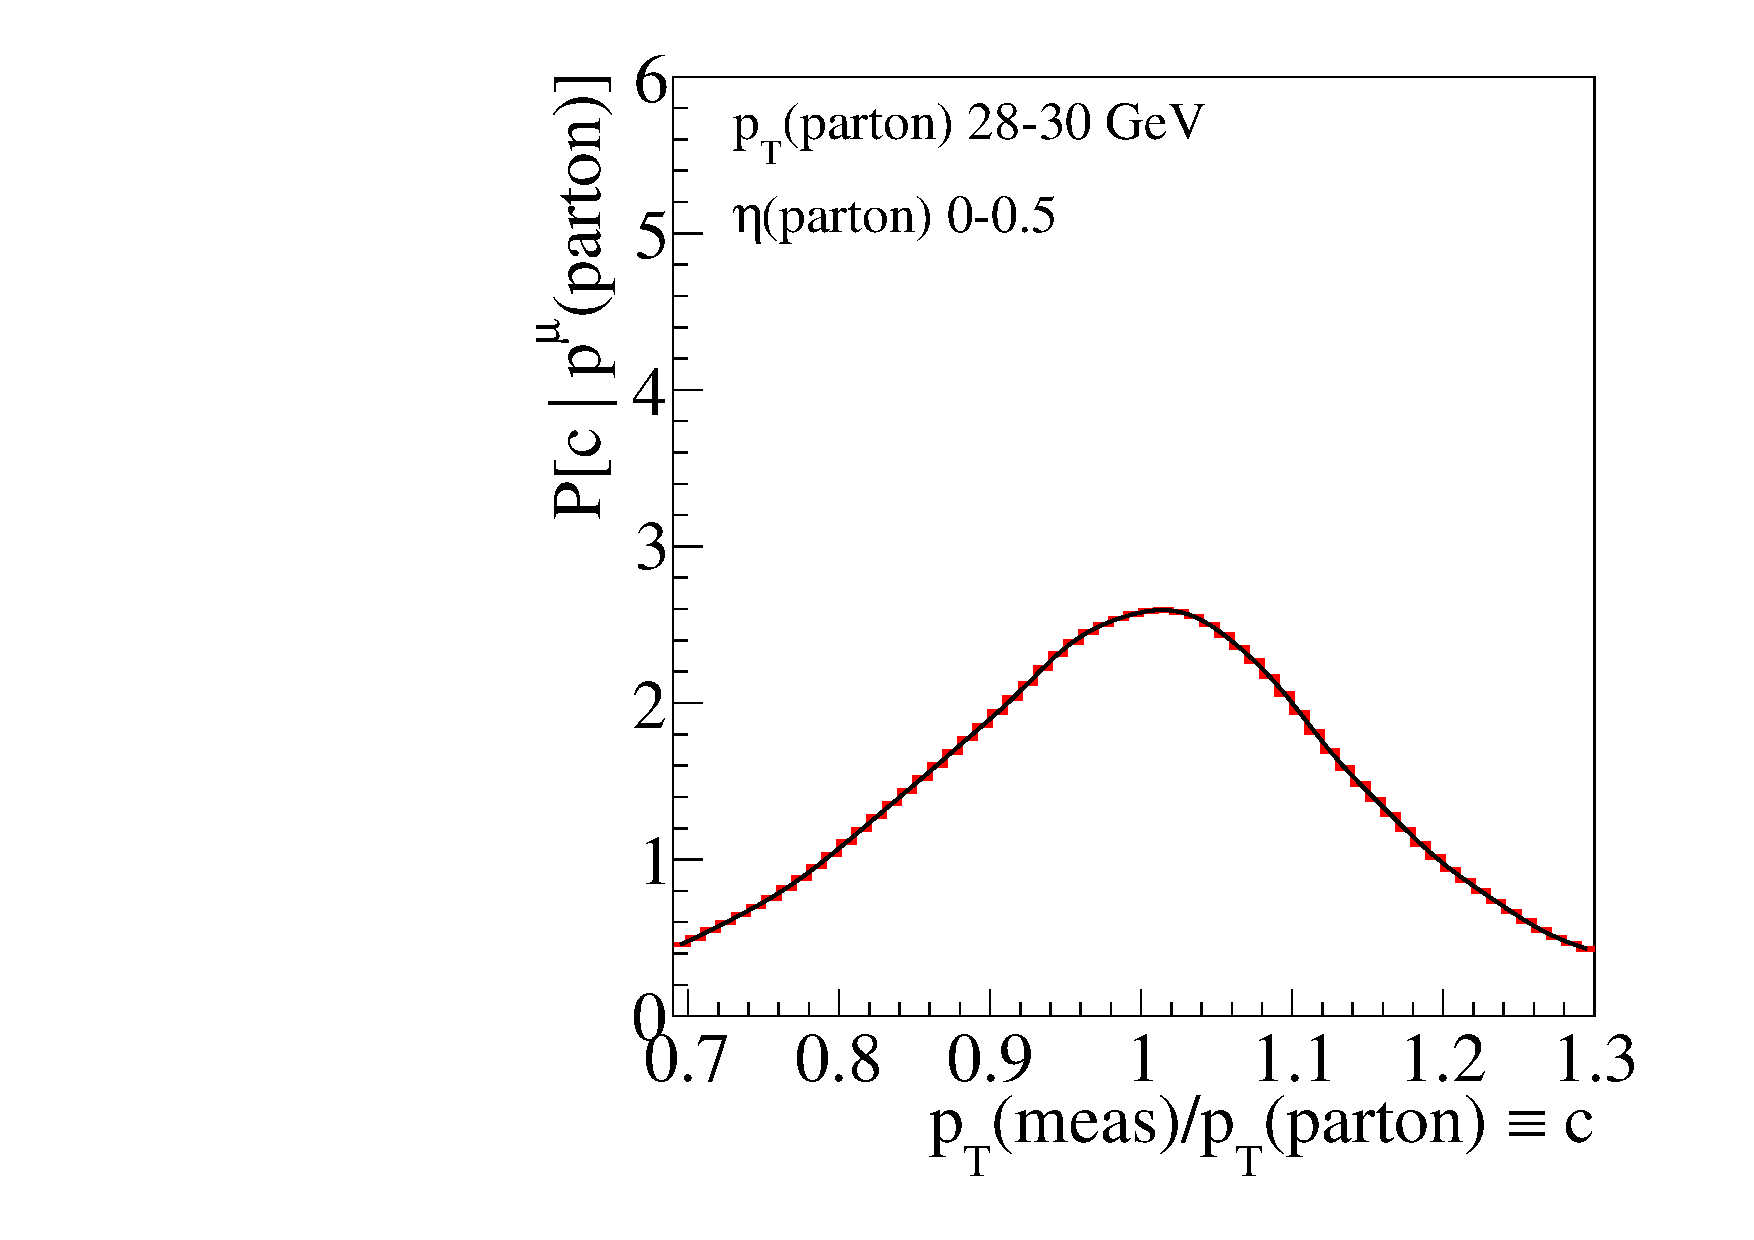
\includegraphics[width=0.5\linewidth]{figures/SusySearches/Ra2b2016/SmearEx1.pdf}
}
\subfloat[]{
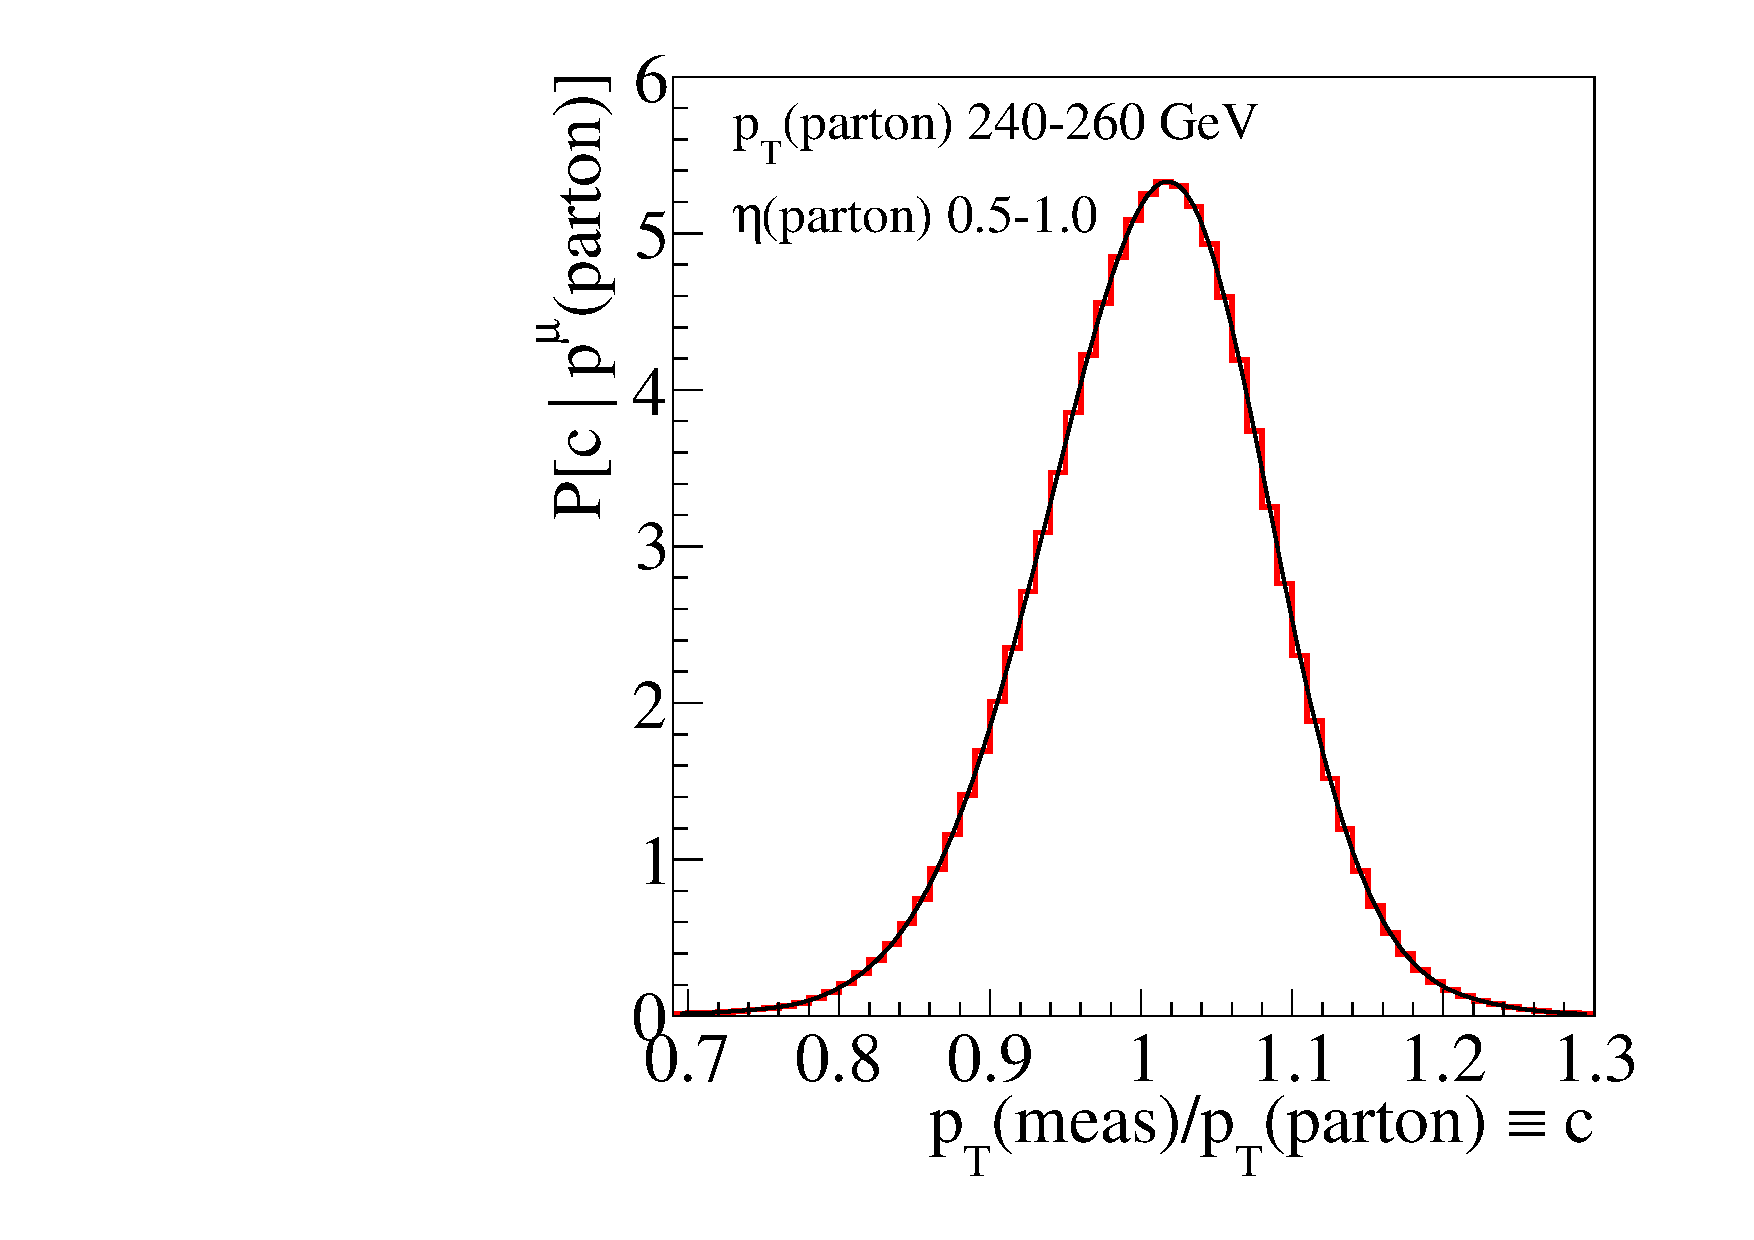
\includegraphics[width=0.5\linewidth]{figures/SusySearches/Ra2b2016/SmearEx2.pdf}
}
\caption{The likelihood function for the jet energy scale factor in two regions of the phase space of the parton-level jet four-vector. These distributions are equivalent to the smearing templates. The histograms (red) are smoothly interpolated using splines (black).}
\label{fig:SmearEx}
\end{figure}


\subsection{Rebalance and smear method}
The rebalance and smear method, originally developed by the authors of the Dissertations~\cite{Koay:2011qqa}\cite{Schroder:2012lqa}\cite{Goebel:2015kca} and the paper~\cite{Chatrchyan:2014lfa}, exploits the relationships given in Equations \ref{eq:metTrue}, along with the jet energy resolution, to form a transfer function between the measured and parton-level jets. The first step of the method is to identify the optimal matrix of scale factors $\hat{C}$ that transforms the collection of reconstruction-level jets into a set that resembles a parton-level jet collection, and (historically) yields an event with $\mht=0$; jets in the resulting collection are referred to as the rebalanced jets. In the second step, the four-vectors of the rebalanced jets are smeared according to the likelihood for the scale factor given in Equation \ref{eq:JetEnergyLikelihood}; events can be smeared as many times as is necessary to make predictions in all signal regions. The above procedure, applied to all events in a QCD-enriched data control sample, yields an event sample that is the basis of the QCD background prediction. Predictions for the QCD background in the signal regions are derived from cuts applied to this sample, which we may refer to as the prediction event sample. I have adapted key aspects of the methodology, which I will now describe step-by-step.

\subsubsection{Rebalance procedure: a Bayesian approach}
The objective is to rebalance the collection of measured jets so that it resembles a parton-level collection. In the re-envisioned approach,  it is possible to systematically  incorporate prior knowledge about the true $\mht$ distribution and jet response functions to constrain the jets.  An inversion of the likelihood function for the jet energy scale factors is performed using Bayes' theorem (see Chapter \ref{chap:run1pmssm} for a brief introduction). The probability density for the parton-level jet collection can be written as
\begin{equation}
{\rm P}(\vec{J}_{\rm part}|\vec{J}_{\rm meas}) \sim {\rm P}(\vec{J}_{\rm meas}|\vec{J}_{\rm part})\cdot \pi(\vec{J}_{\rm part}),
\label{eq:posterior1}
\end{equation}
where $\pi(\vec{J}_{\rm part})$ is the $n$-dimensional prior probability density for the parton-level jet collection.
Treating the jets as mutually independent allows the likelihood to be factorized as
\begin{align}
\begin{split}
{\rm P}(\vec{J}_{\rm meas}|\vec{J}_{\rm part}) = \prod_{i=1}^{\njets}L_{i} &= \prod_{i=1}^{\njets}{\rm P}(p^{\mu}_{i,\rm meas}\ |\ p^{\mu}_{i,\rm part})\\
&=\prod_{i=1}^{\njets}{\rm P}(c_i\ |\ p^{\mu}_{i,\rm part}).
\end{split}
\label{eq:likelihood1}
\end{align}
The prior allows our knowledge about the parton-level missing transverse energy outlined in Equation \ref{eq:metTrue} to constrain of the jets. However, while equations \ref{eq:metTrue} are true for the $E_{T}^{\rm miss}$, high pileup conditions necessitate the use of the so-called missing transverse hadronic energy $\mht$, defined as
\begin{equation}
\vec{H}_{T}^{\rm miss} \equiv -\sum_{i=1}^{{\rm N}_{\rm jet}}(\vec{p}_{T})_{i}\cdot\Theta(30{\rm\ GeV}-(p_{T})_{i}).
\end{equation}
The threshold on the $p_{T}$ applied via the Heaviside function to remove jets originating from pileup interactions spoils the equality in Equation \ref{eq:metTrue}. Jets with $p_{T}$ less than 30 GeV can recoil off harder jets, and this produces non-zero true $\mht$. However, the parton-level $\mht$ is still small compared to the reconstruction-level $\mht$, as seen in the distribution of parton- and reconstruction-level $\mht$ in Fig. \ref{fig:Mht}, implying that the underlying $\mht$ distribution may provide a meaningful constraint on our knowledge of the parton-level system. A difference is also seen in the angular distribution of the $\mht$, in the polar coordinate system with the z-axis defined along the direction of the leading jet, and this information is likewise incorporated.
\begin{figure}[h]
\centering
\subfloat[]{
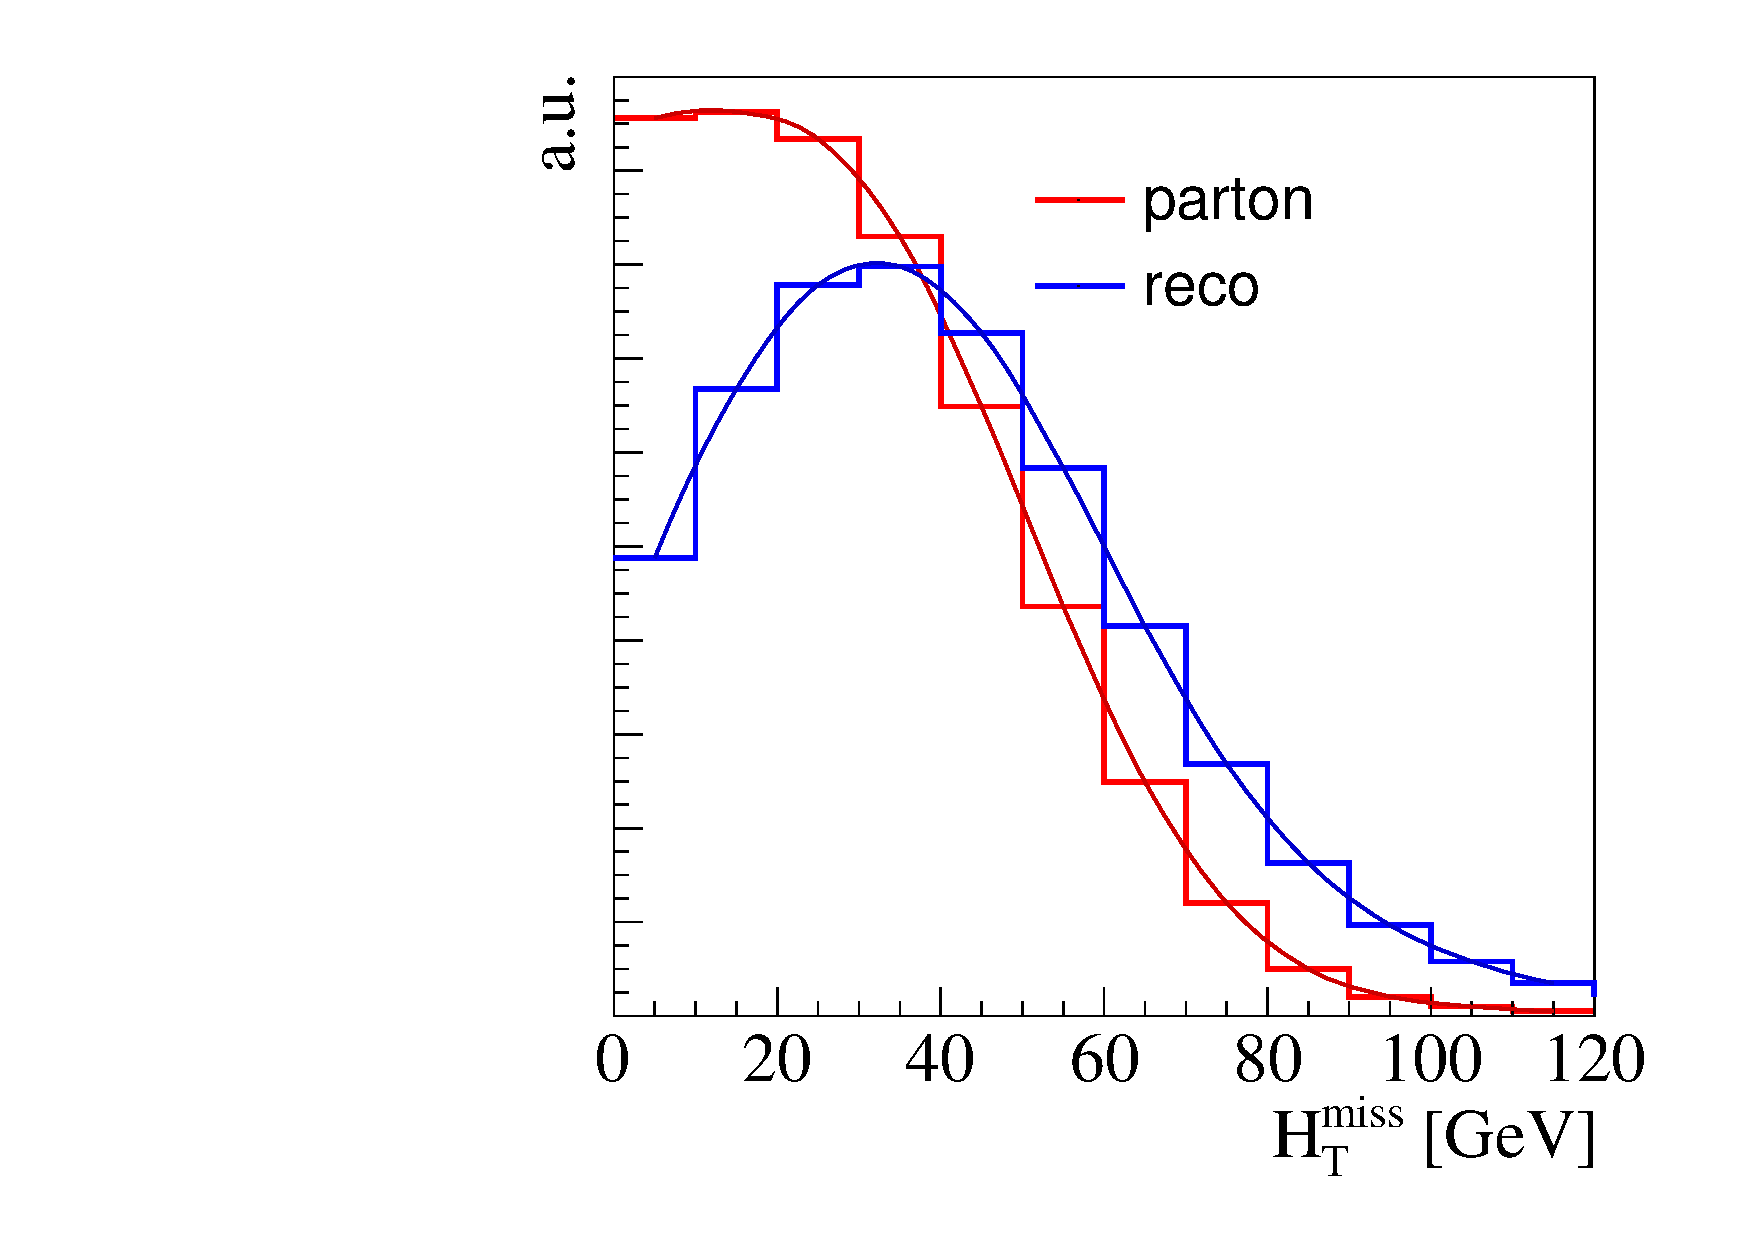
\includegraphics[width=0.5\linewidth]{figures/SusySearches/Ra2b2016/MhtGenAndTruth.pdf}
}
\subfloat[]{
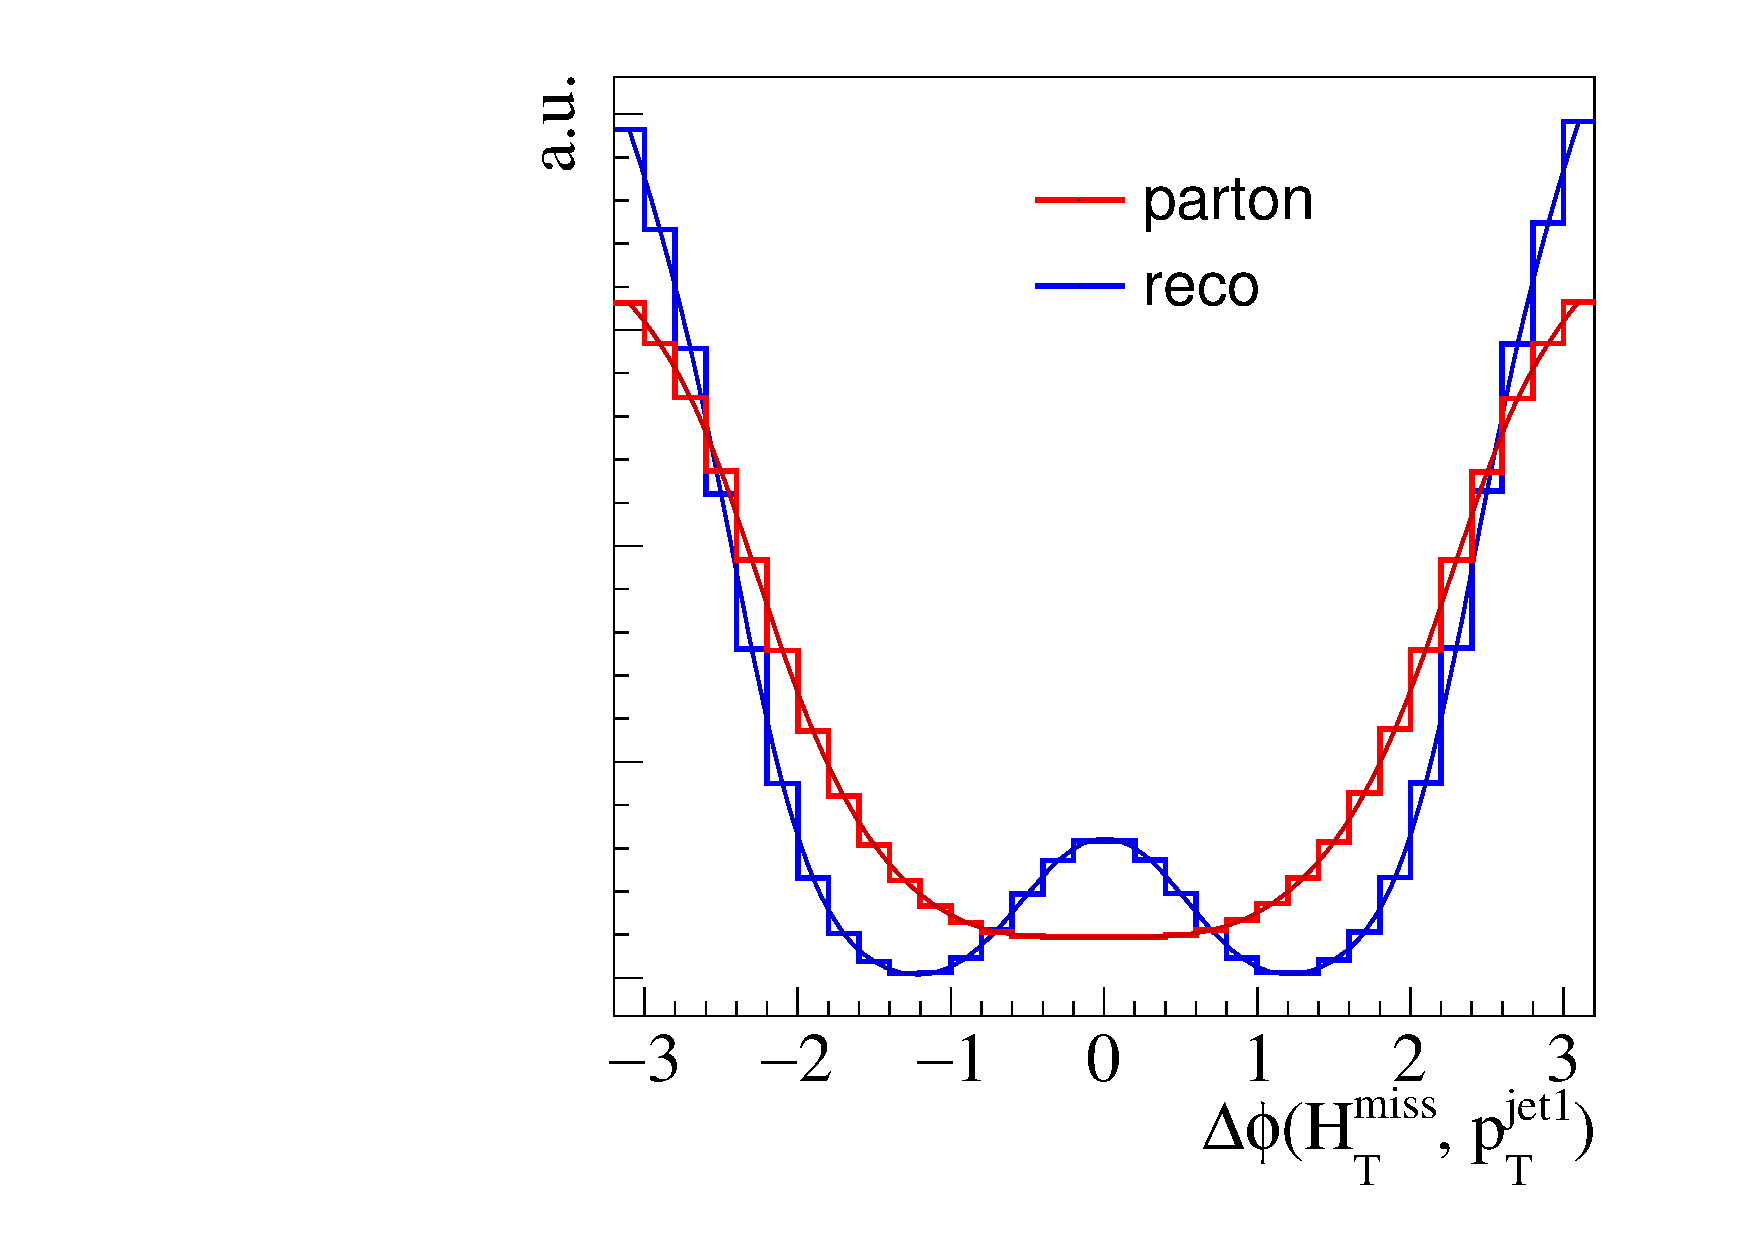
\includegraphics[width=0.5\linewidth]{figures/SusySearches/Ra2b2016/DPhiMhtJet1GenAndTruth.pdf}
}
\caption{The parton-level and reconstruction-level $\mht$ and azimuthal separation between the $\mht$ and leading jet in QCD simulation. The red functions are taken as probability distributions making up the prior, $\text{P}[\mht(\vec{J}_{\rm part})]$ and $\text{P}[\Delta\phi_{\mht,p_{T}^1}(\vec{J}_{\rm part})]$}
\label{fig:Mht}
\end{figure}

The expression relating the parton-level $\mht$ to the jet energy scale factors is used, in conjunction with the red probability densities, to form factors in the prior. The templates for the $\Delta\phi$ between the $\mht$ and the leading jet are derived separately in bins of the b-jet multiplicity, for the bins of 0, 1, and $\geq$ 2 b-jets.  This choice and its implications are discussed later. For the case of one or more b-jets, the $\Delta\phi$ between the $\mht$ and the leading b-jet is used. Combining Eqs. \ref{eq:posterior1} and \ref{eq:likelihood1} gives
\begin{equation}
{\rm P}(\vec{J}_{\rm part}|\vec{J}_{\rm meas}) \sim
\prod_{i=1}^{\njets}{\rm P}(p^{\mu}_{i,\rm meas}|p^{\mu}_{i,\rm part})\cdot \text{P}[\mht(\vec{J}_{\rm part})]\cdot \text{P}[\Delta\phi_{\mht,p_{T}^1}(\vec{J}_{\rm part})]\cdot \pi_0(\vec{J}_{\rm part}),
\end{equation}
where $\pi_0(\vec{J}_{\rm part})$ is the initial prior on the parton jet four-vectors, taken to be uniform. Having constructed a posterior density, the parton-level jets are inferred by integrating with respect to the reconstruction-level jet four-vectors, or alternatively, by performing a likelihood maximization. The second approach is taken.


\subsubsection{Posterior density of jet momenta}
Bayes' theorem suggests that incorporating new relevant information will lead to improved knowledge about a system. In the case of the rebalance and smear method, a rebalanced event is expected to more closely resemble the parton-level event than does the reconstruction-level event. Figure \ref{fig:rebareso} shows that the resolution of rebalanced jets is better than that of reconstructed jets by approximately 10\%.
\begin{figure}[h]
\centering
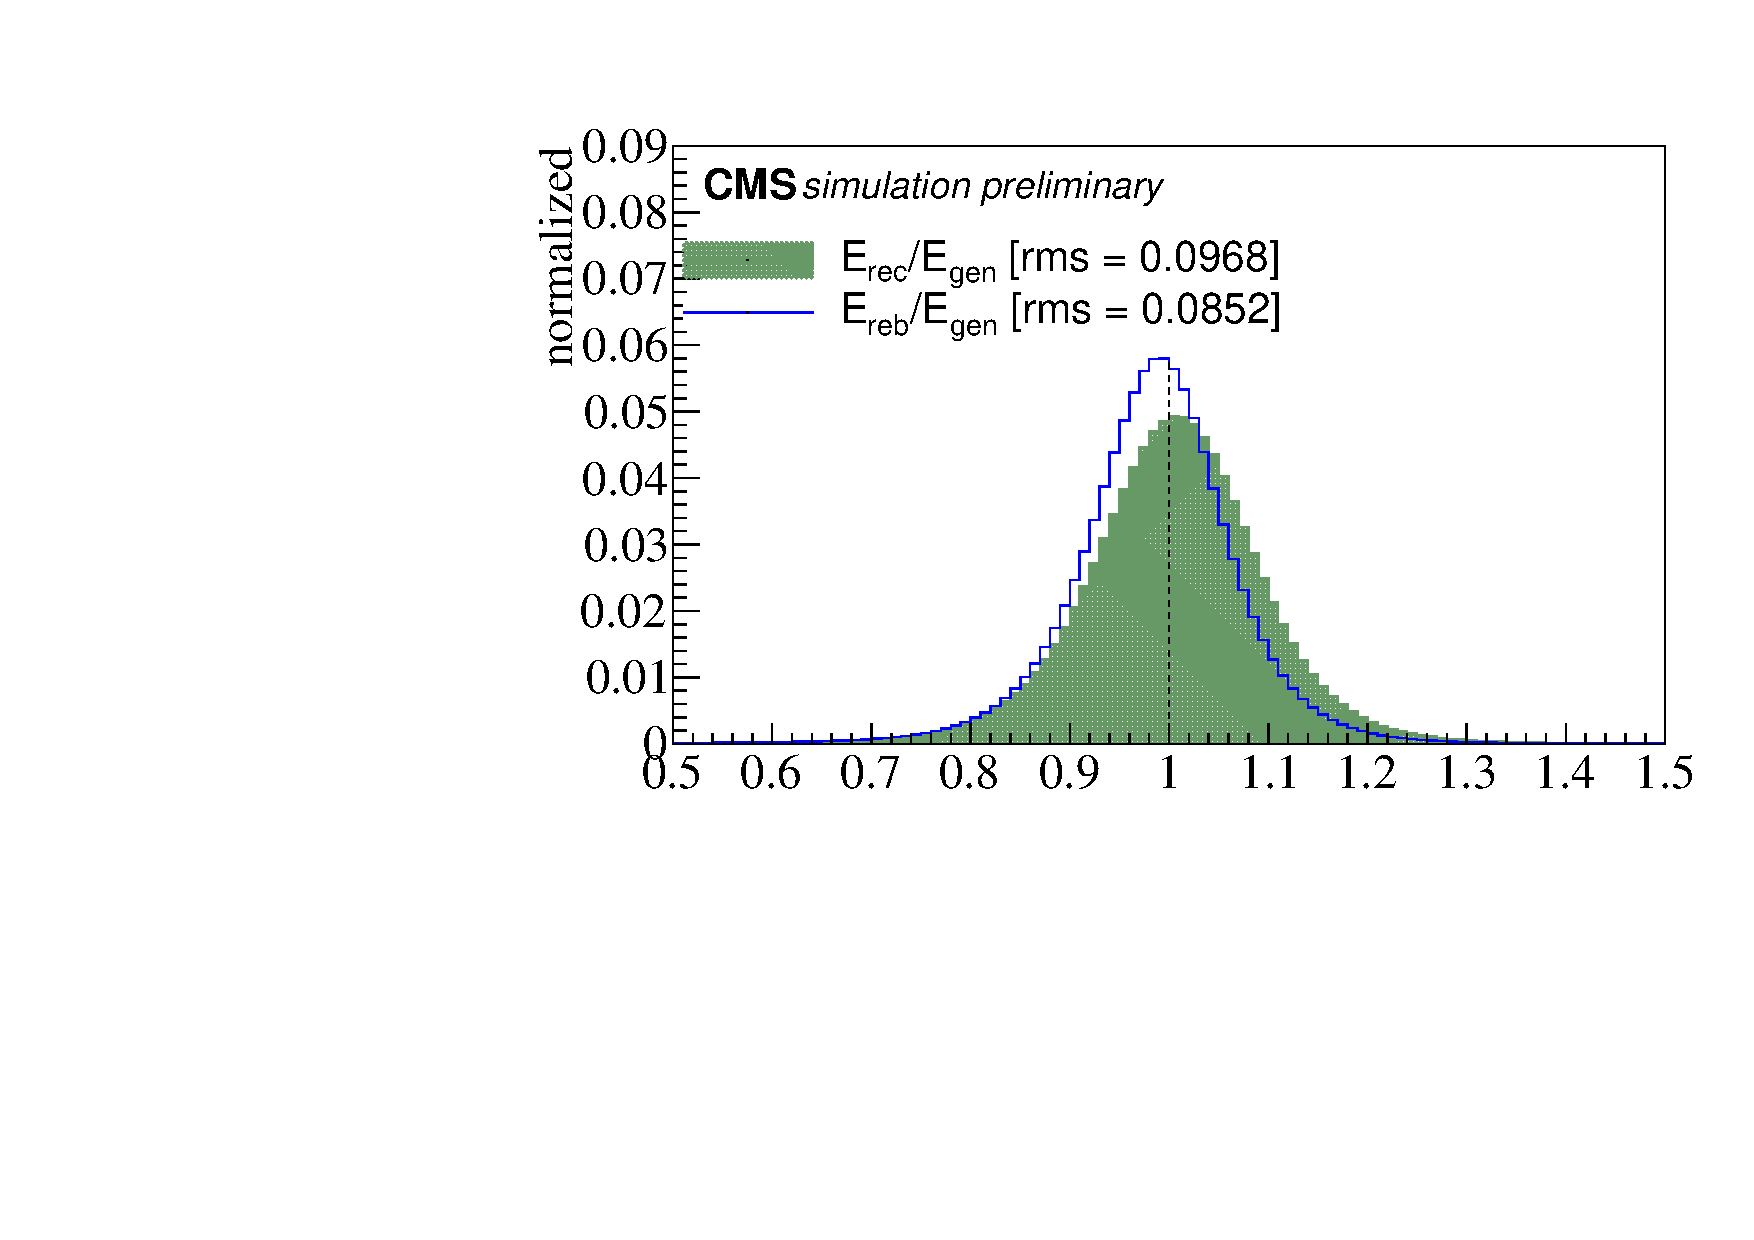
\includegraphics[width=0.49\linewidth]{figures/SusySearches/Ra2b2016/Jet1Resolution.pdf}
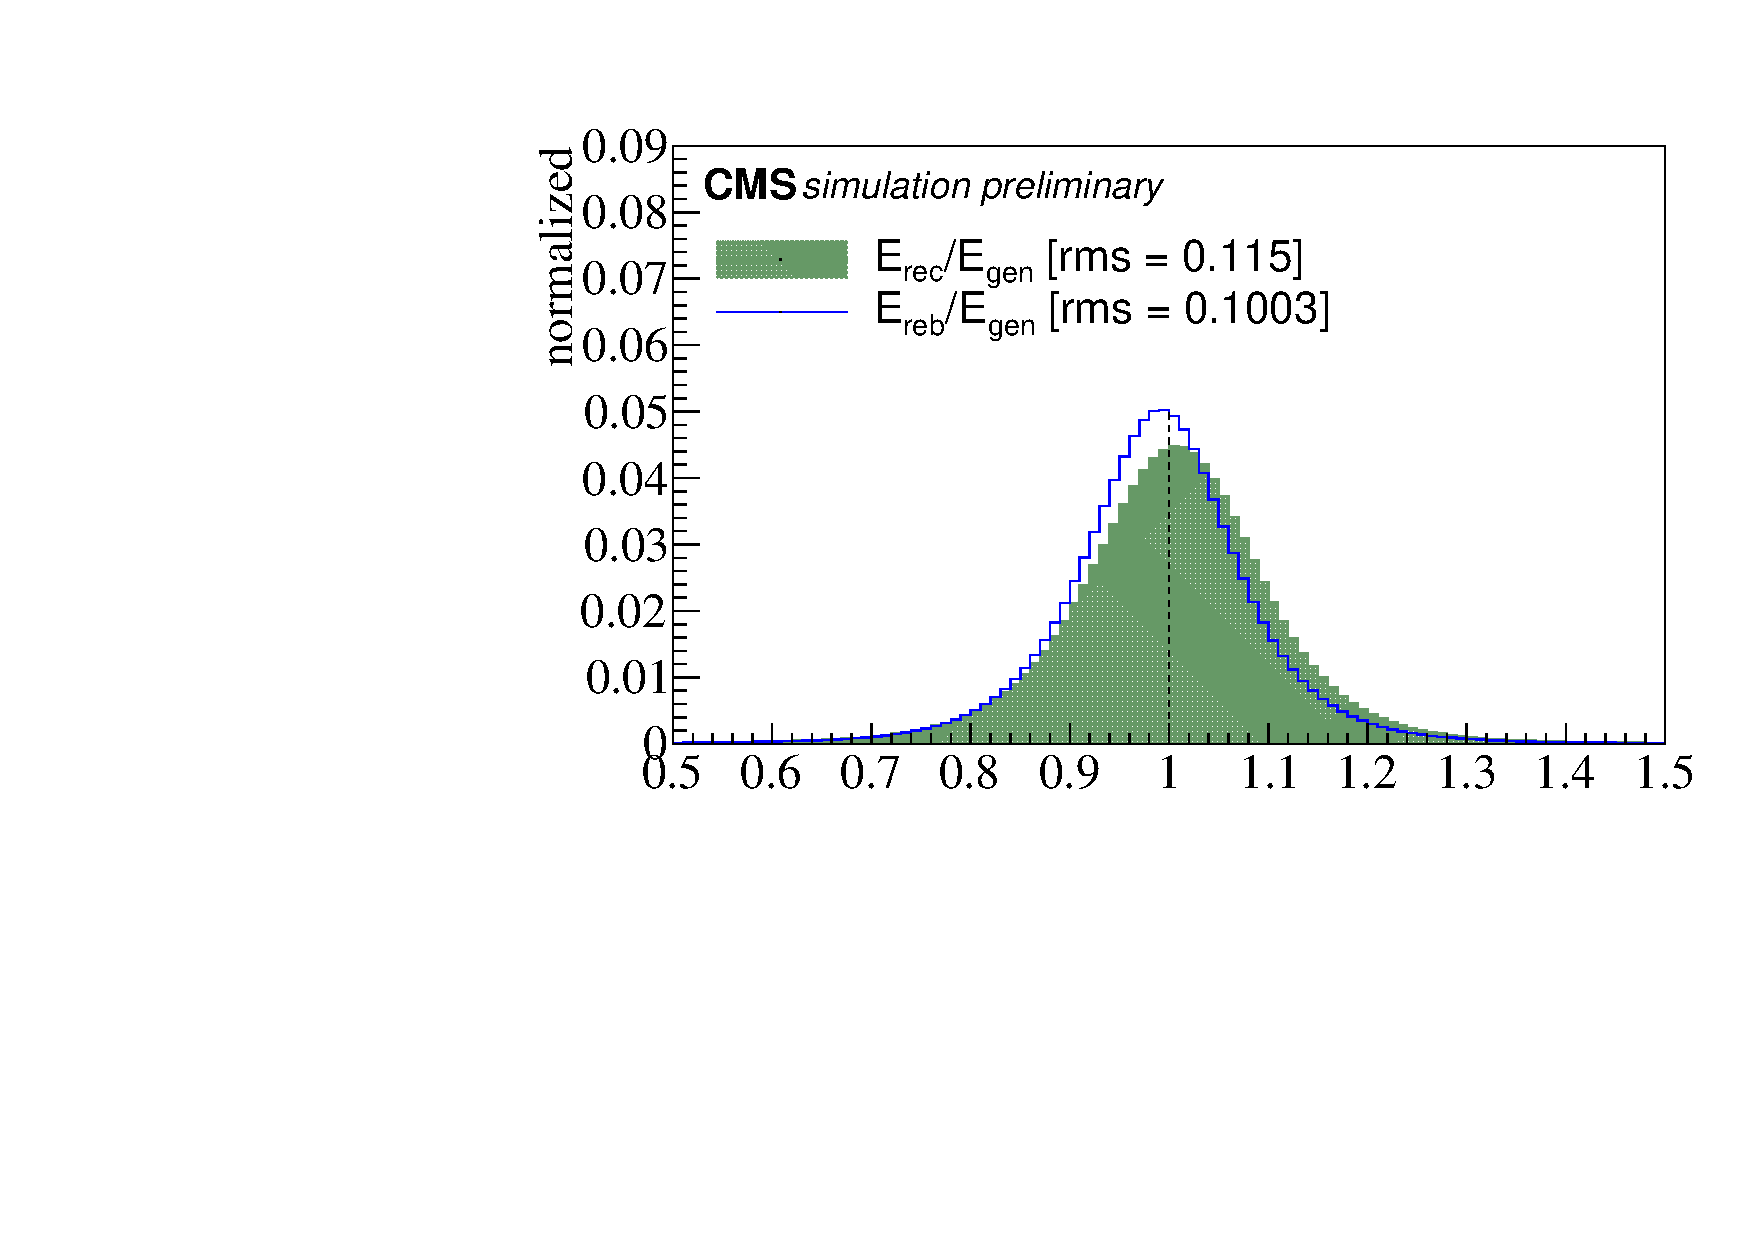
\includegraphics[width=0.49\linewidth]{figures/SusySearches/Ra2b2016/Jet2Resolution.pdf}
\caption{The jet energy response for the leading jet (left) and sub-leading jet (right) for reconstructed jets (green) and rebalanced jets (blue). Parton-level jets are required to have $\pt>30$ GeV and $|\eta|<2.4$. The resolution of rebalanced jets is better (smaller) than that of reconstruction-level jets by bout 10\%.}
\label{fig:rebareso}
\end{figure}
We also observe the peak of the response to be slightly lower for rebalanced jets than for reconstructed jets. This is consistent with the peak of the jet $\pt$ likelihood functions being centered at values slightly higher than 1, as seen in Fig. \ref{fig:SmearEx}. 
\FloatBarrier

\subsection{Closure}
The rebalance and smear prediction is applied to simulated events and compared with the result obtained directly from the simulation. A set of baseline selection, similar to that applied in the search \cite{Khachatryan:2016kdk}, is applied. Events are required to have:
\begin{itemize}
\item no reconstructed, isolated particle track with a $\pt>10$ GeV and $|\eta|<2.4$;
\item $\Ht>500$ GeV;
\item $\mht>150$ GeV;
\item $\njets\geq$ 4, where jets are required to have a $\pt>30$ GeV and $|\eta|<2.4$, and pass a loose set of quality selection criteria.
\item an azimuthal separation between the $\mht$ and the leading four jets $\Delta\phi(\mht$, jet$_{1,2,3,4})>$ 0.5, 0.5, 0.3, 0.3.
\end{itemize}
Figures \ref{fig:BaselineRplusS} through \ref{fig:BaselineRplusS2} show this comparison for a number of observables after the baseline selection of the CMS multi-jet SUSY search, which is described in Section \ref{sec:2015results}. The plots show ``n-1'' distributions, meaning all baseline selection have been applied except that of the x-axis variable. Then, Figs. \ref{fig:LowDeltaPhiRplusS} through \ref{fig:LowDeltaPhiRplusS2} show the comparison in an inverted $\Delta \phi$ region that has a selection equivalent to the baseline but with the selection on the $\Delta \phi$ between the $\mht$ and the jets inverted. Figure \ref{fig:RplusSCorrelation} shows the comparison in two dimensions for selected pairs of observables. 

\begin{figure}[h]
\centering
\subfloat[]{
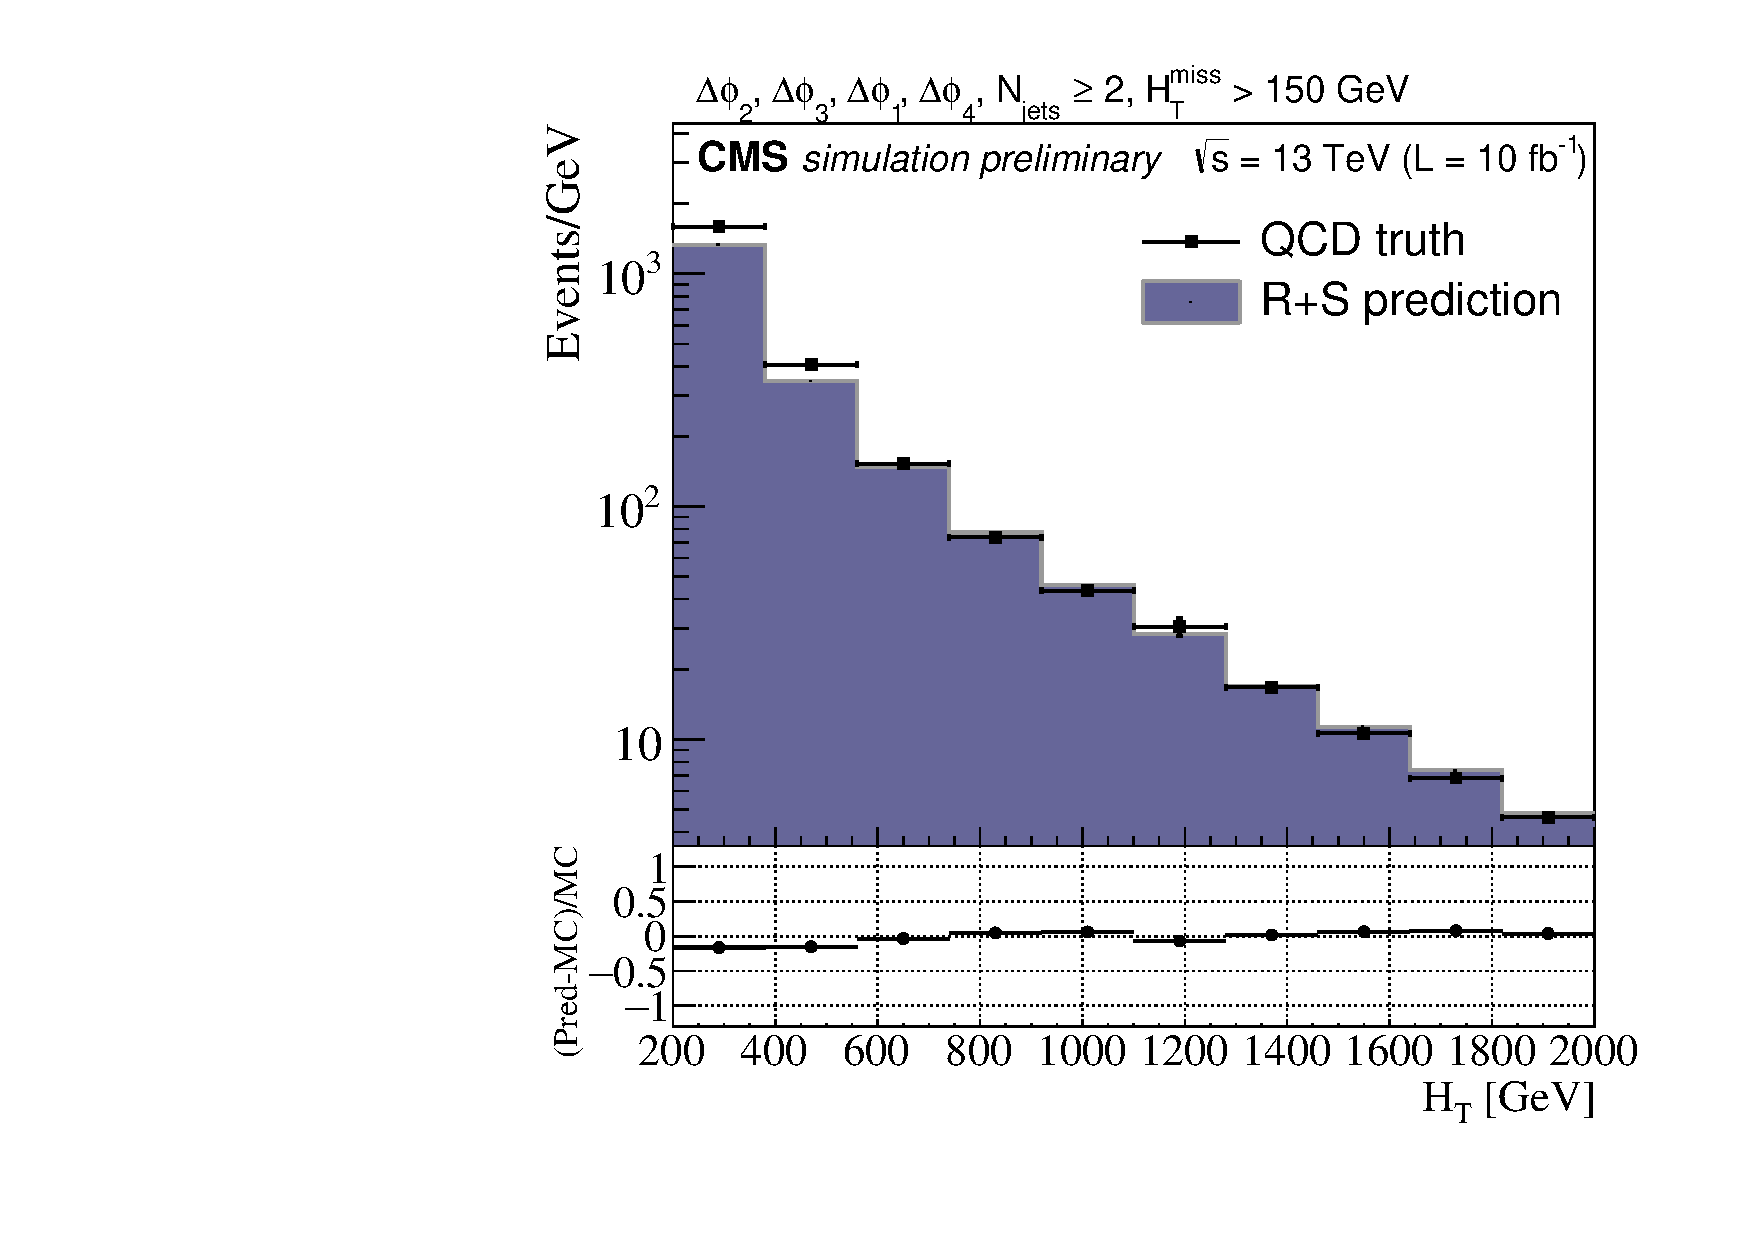
\includegraphics[width=0.5\linewidth]{figures/SusySearches/Ra2b2016/Baseline_Ht.pdf}
}
\subfloat[]{
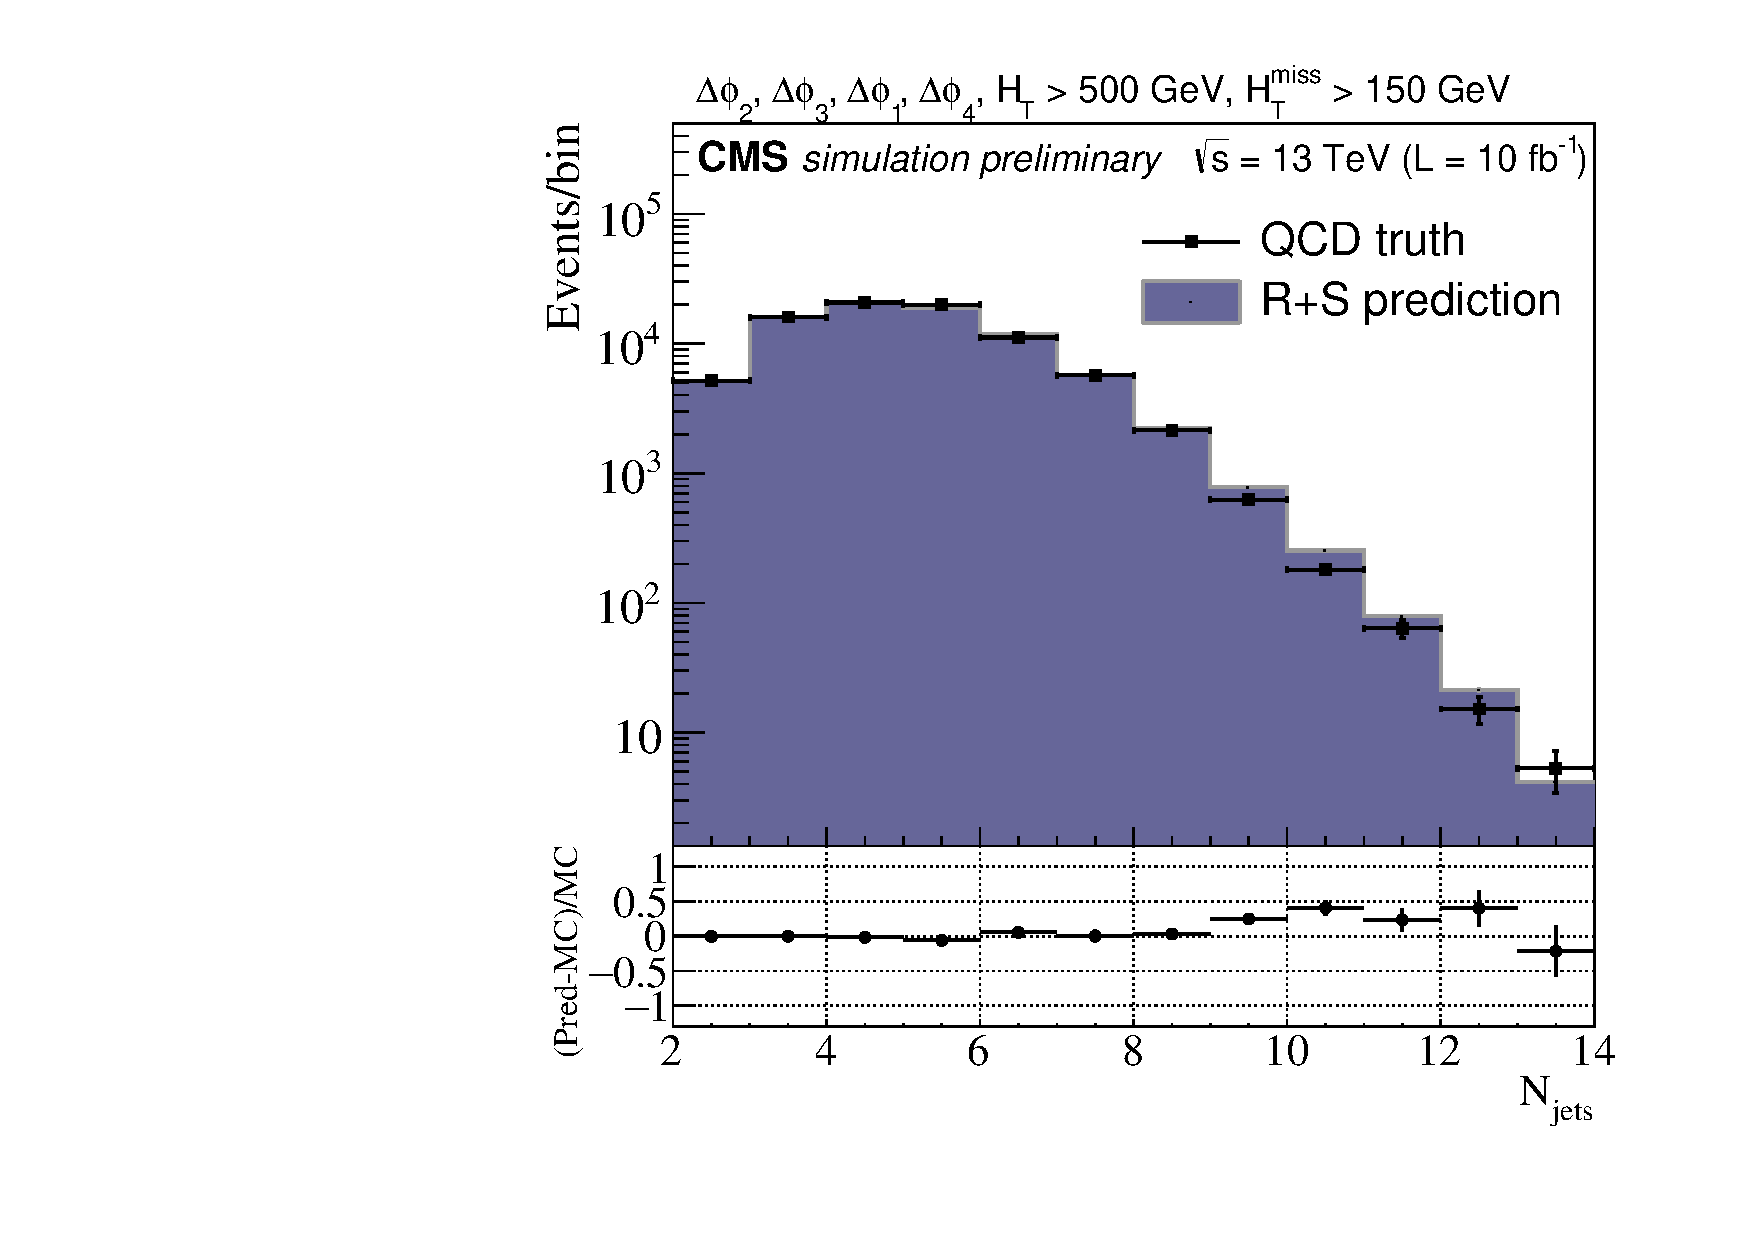
\includegraphics[width=0.5\linewidth]{figures/SusySearches/Ra2b2016/Baseline_NJets.pdf}
}\\
\subfloat[]{
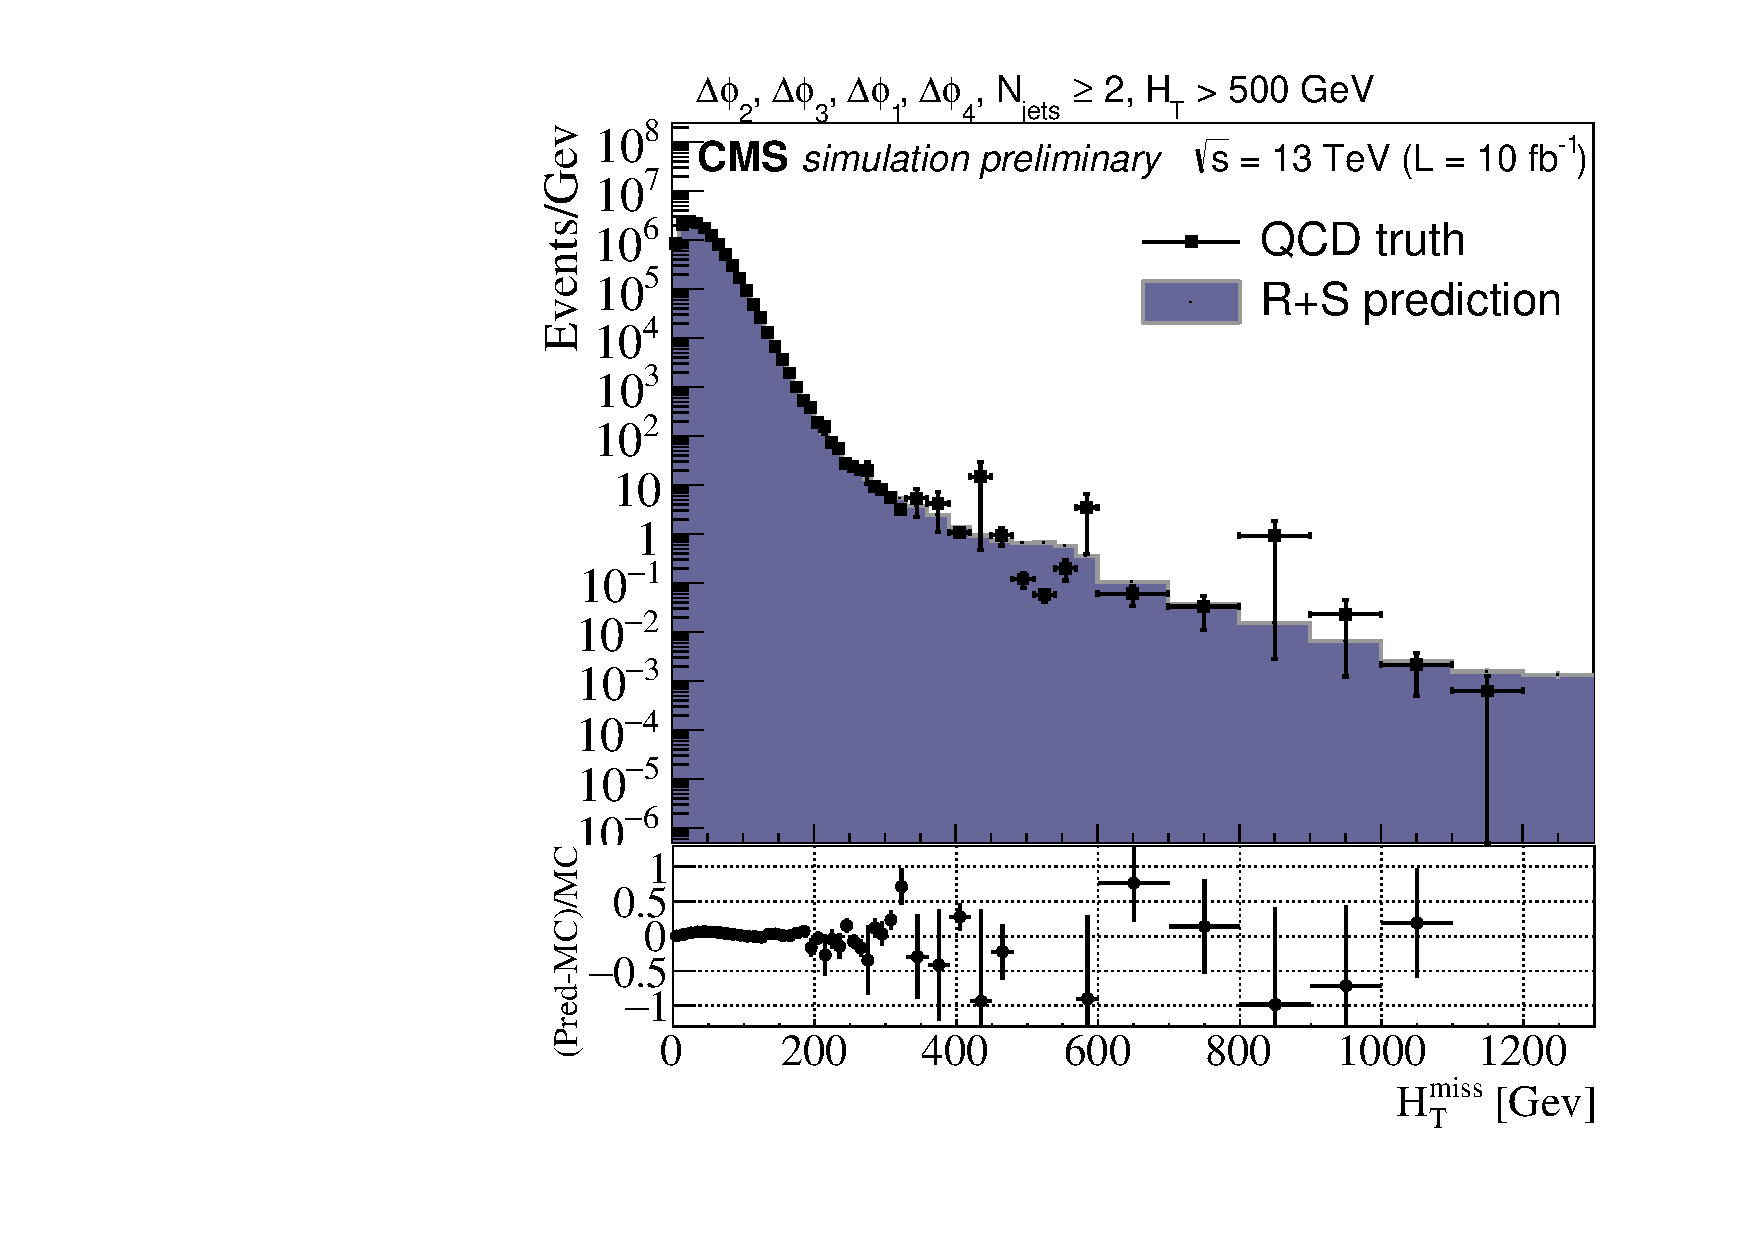
\includegraphics[width=0.5\linewidth]{figures/SusySearches/Ra2b2016/Baseline_Mht.pdf}
}
\subfloat[]{
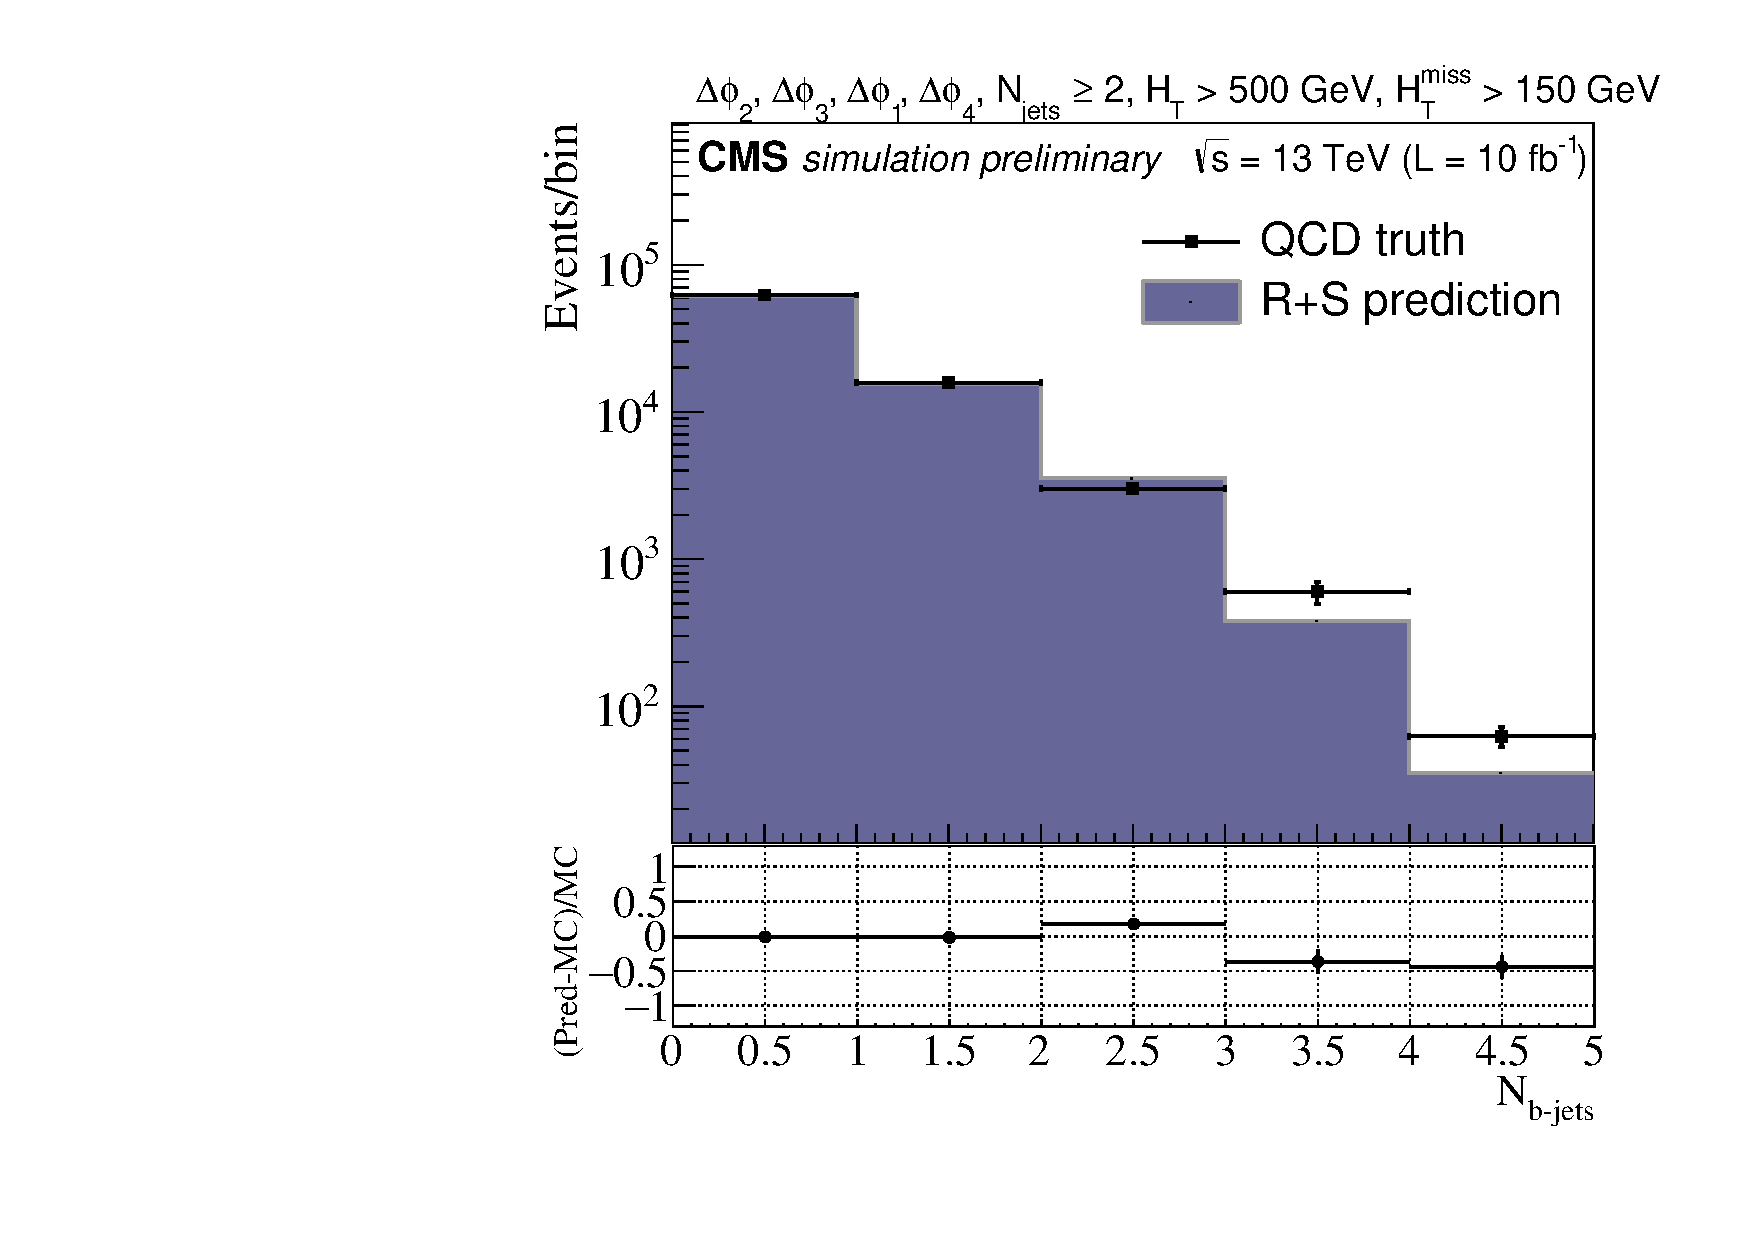
\includegraphics[width=0.5\linewidth]{figures/SusySearches/Ra2b2016/Baseline_BTags.pdf}
}
\caption{Comparisons of kinematic distributions between the direct simulation and the rebalance and smear method applied to simulation, after the baseline selection of the multi-jet SUSY search.}
\label{fig:BaselineRplusS}
\end{figure}


\begin{figure}[h]
\centering
\subfloat[]{
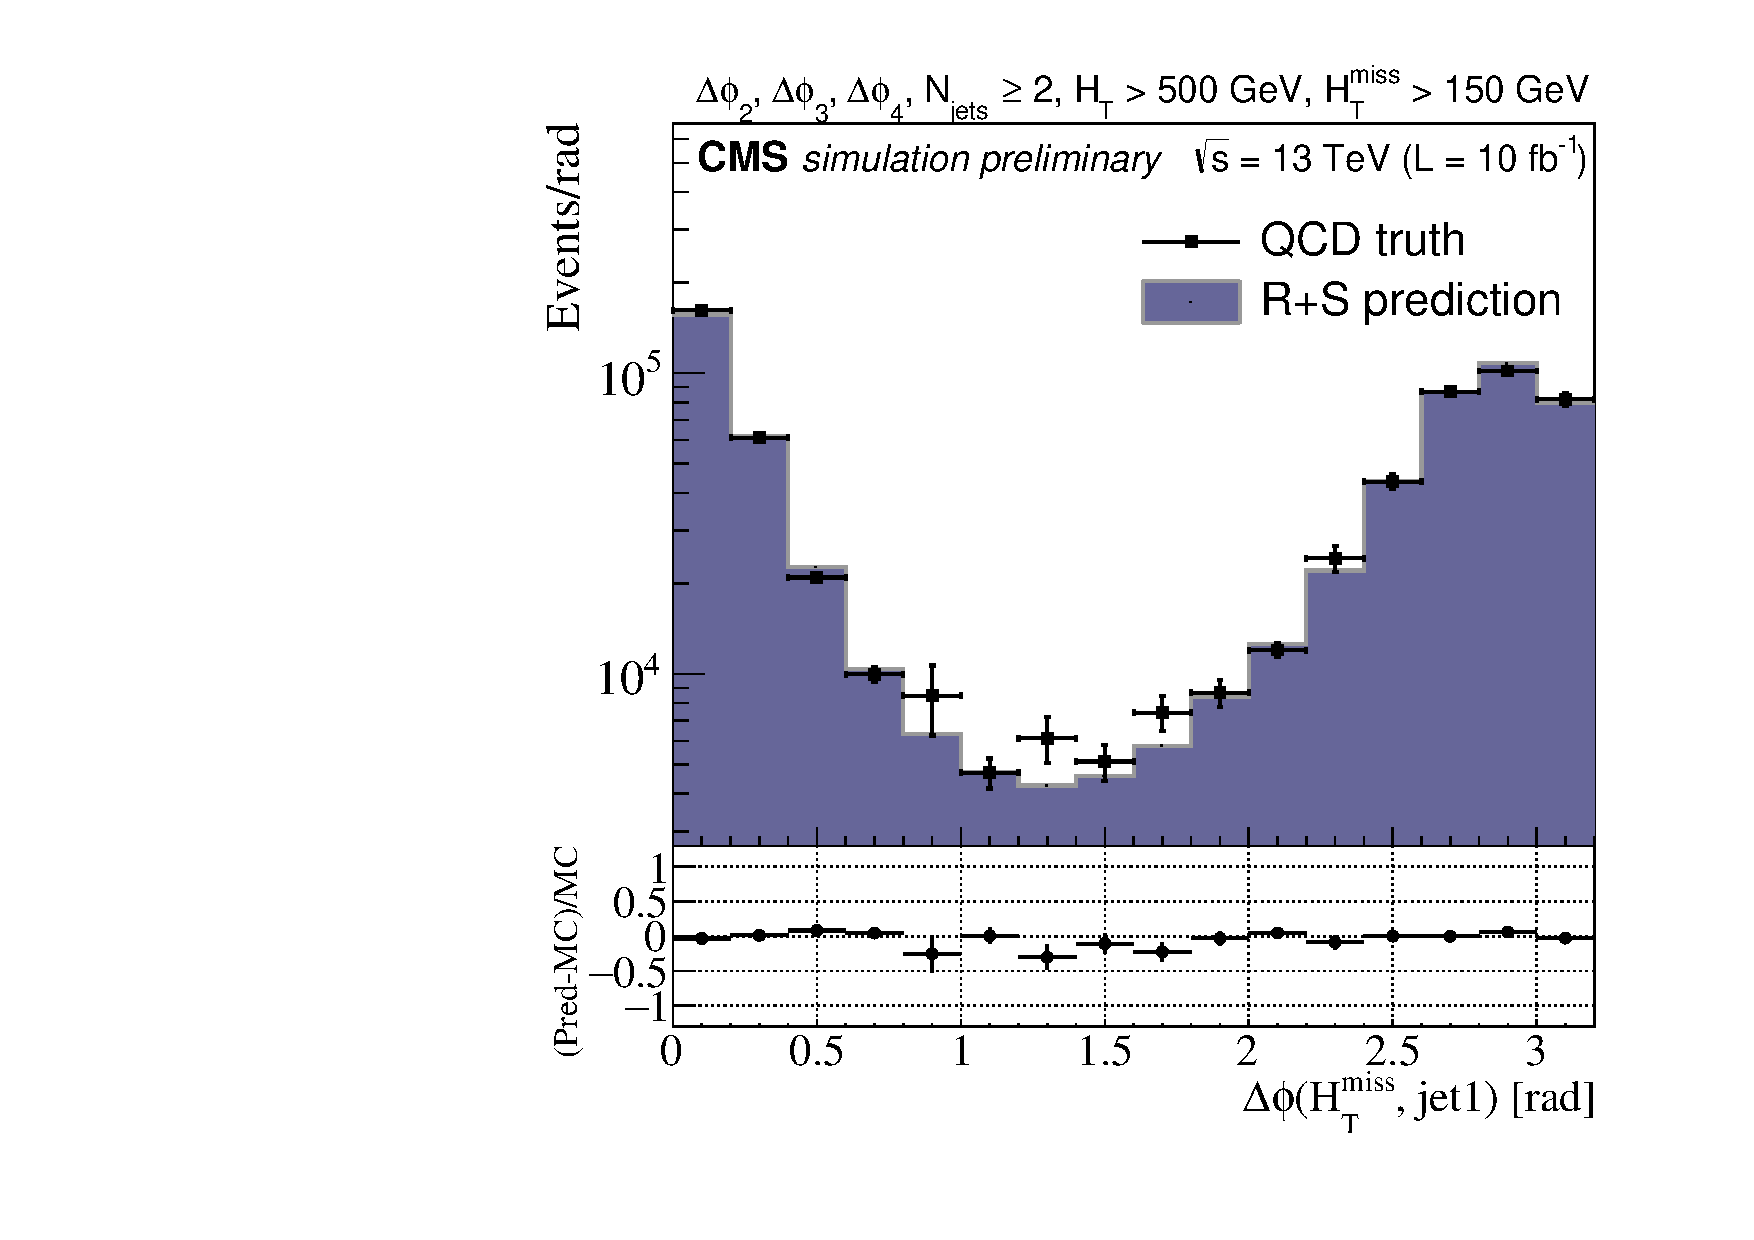
\includegraphics[width=0.5\linewidth]{figures/SusySearches/Ra2b2016/Baseline_DPhi1.pdf}
}
\subfloat[]{
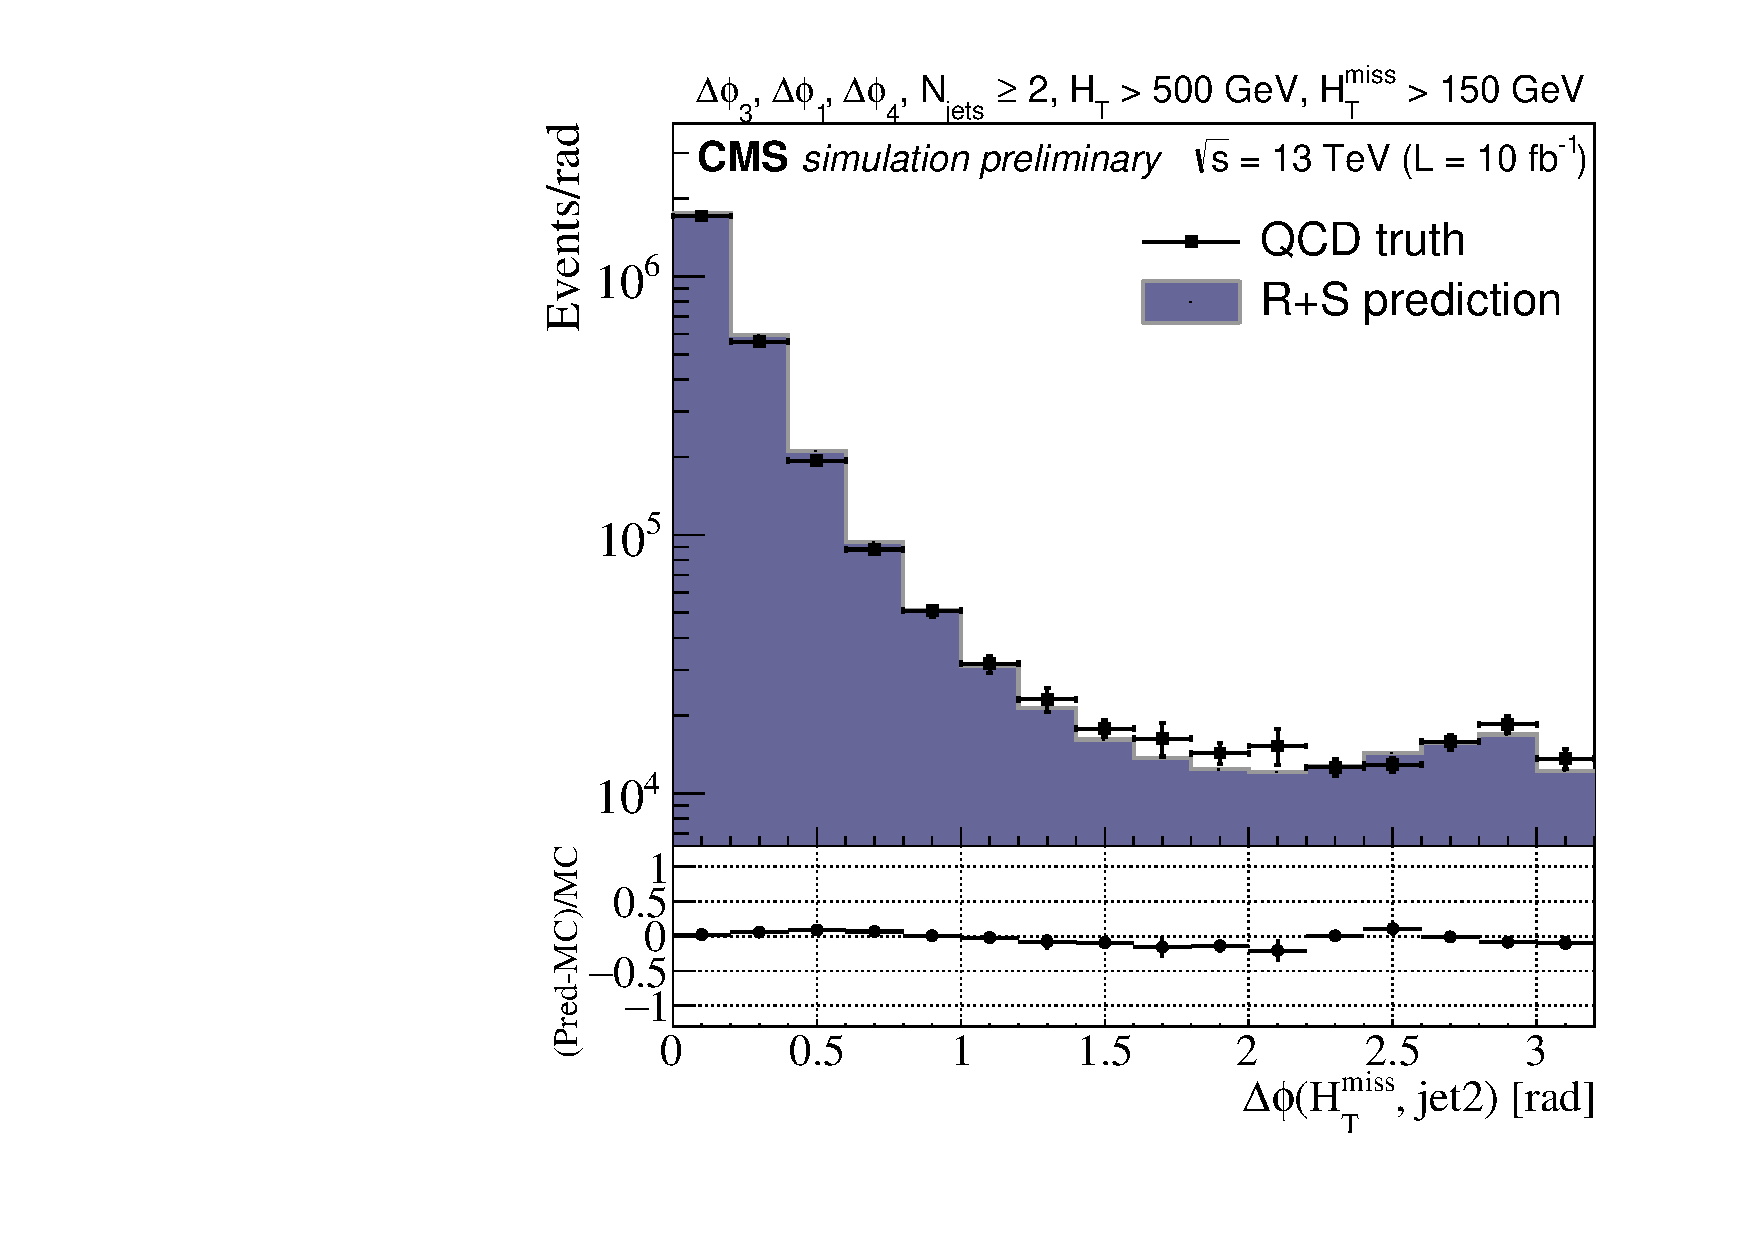
\includegraphics[width=0.5\linewidth]{figures/SusySearches/Ra2b2016/Baseline_DPhi2.pdf}
}\\
\subfloat[]{
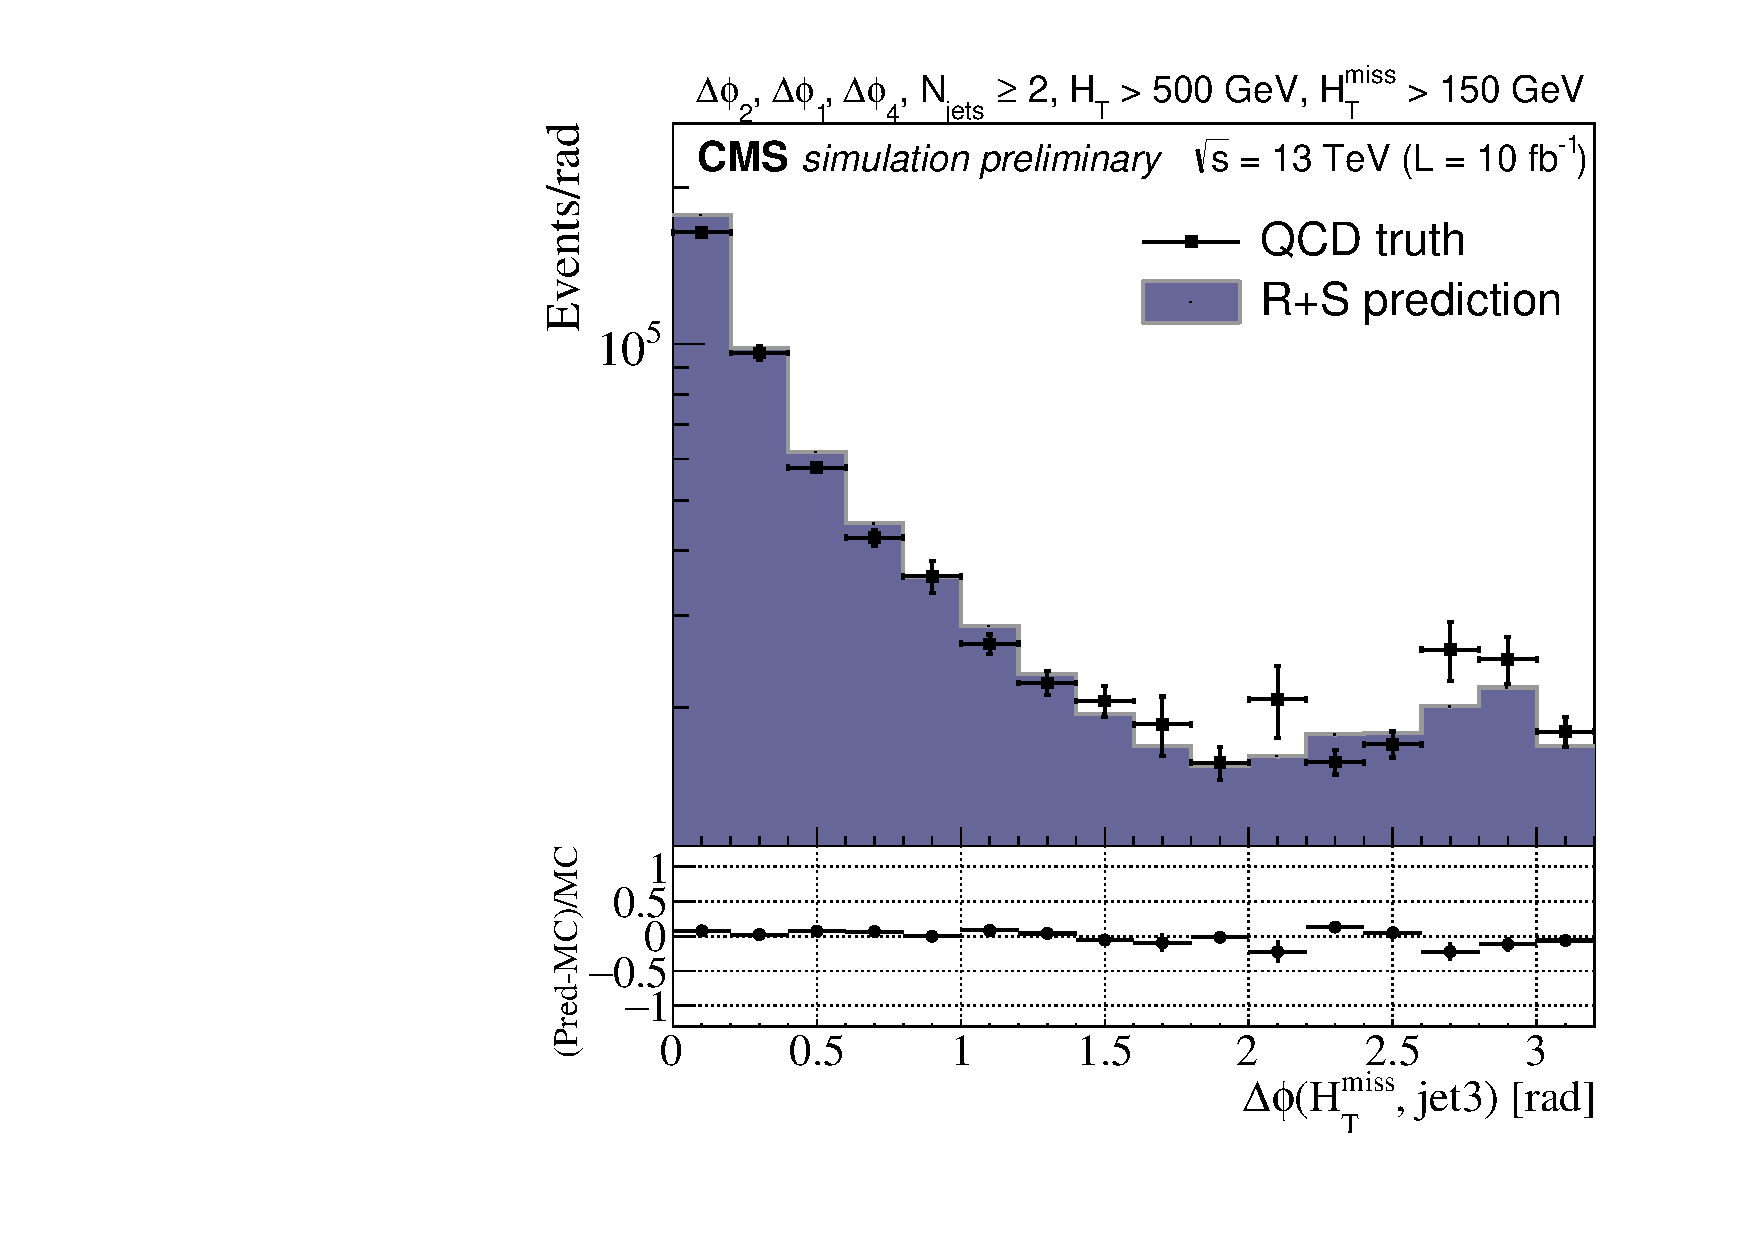
\includegraphics[width=0.5\linewidth]{figures/SusySearches/Ra2b2016/Baseline_DPhi3.pdf}
}
\subfloat[]{
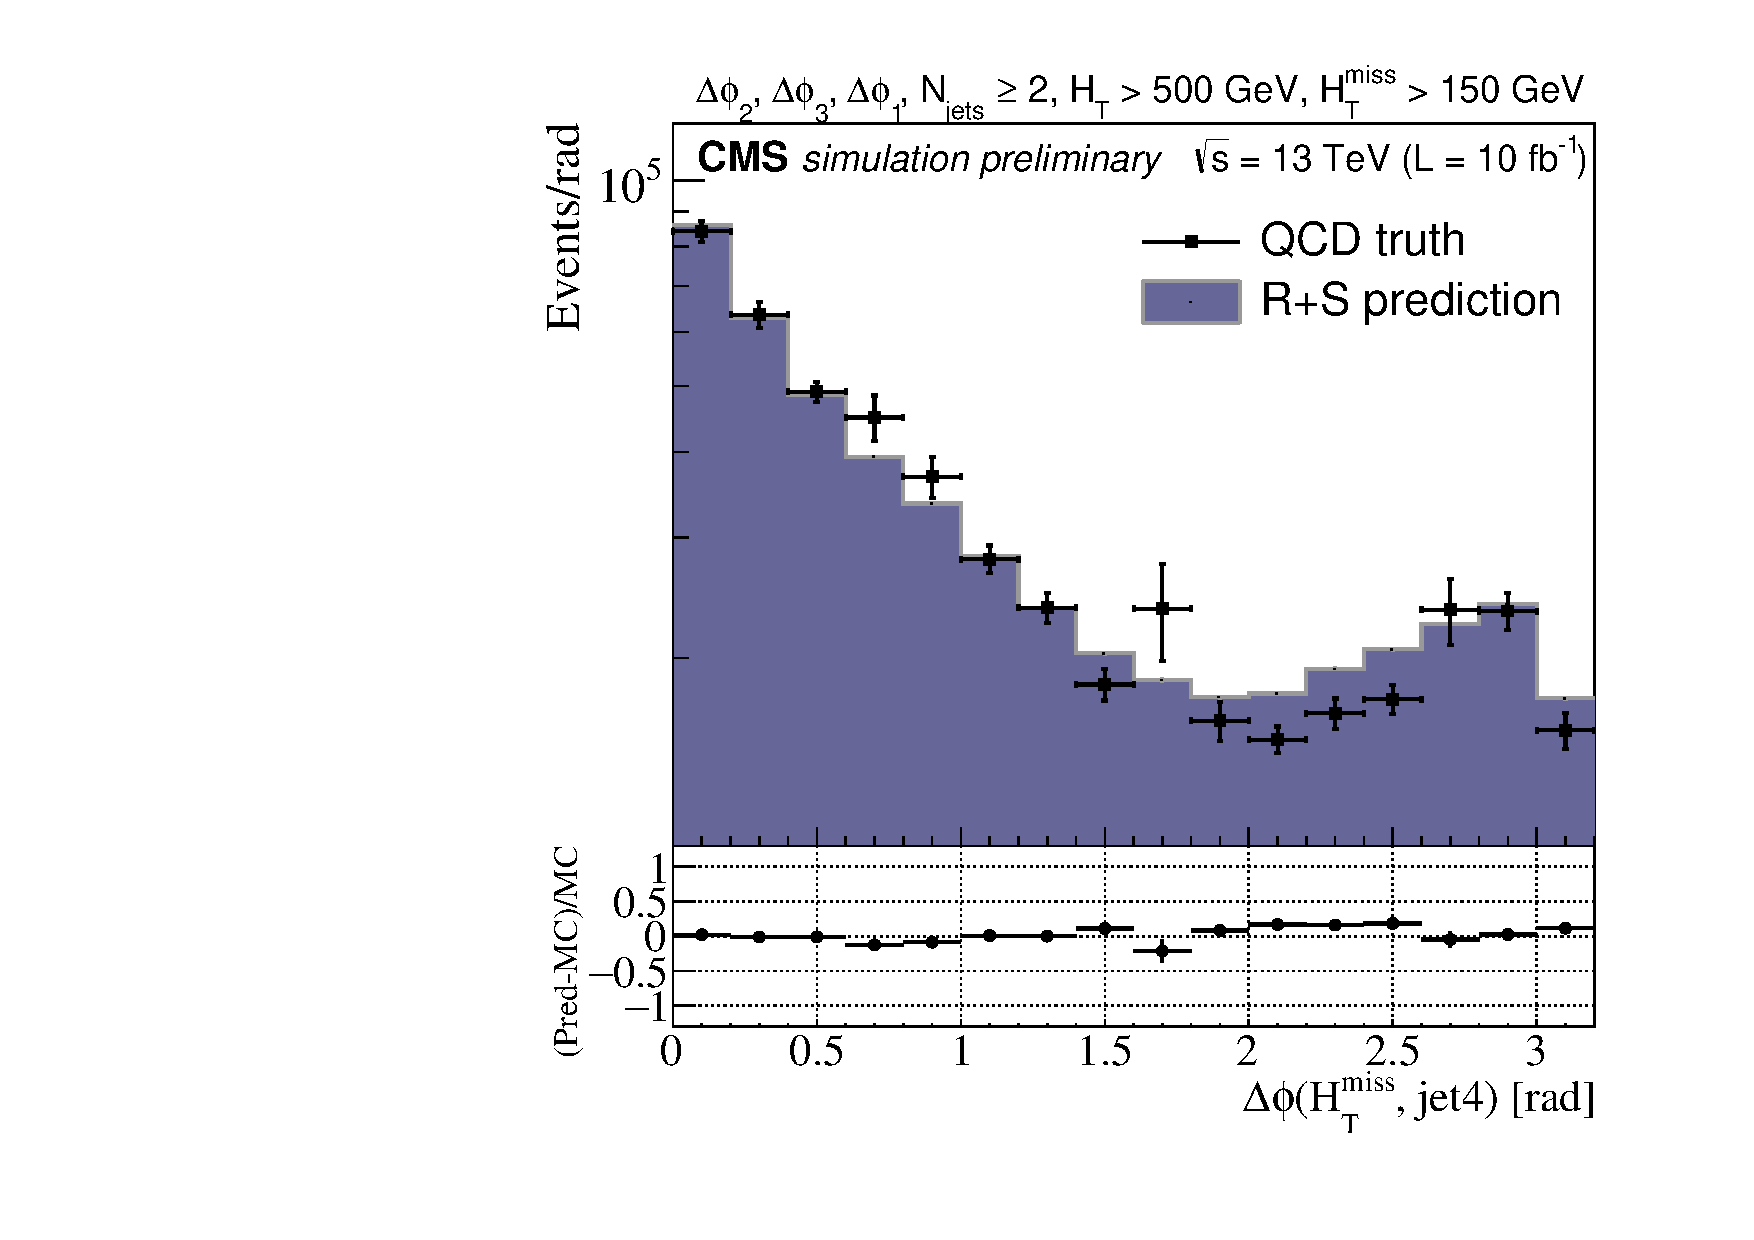
\includegraphics[width=0.5\linewidth]{figures/SusySearches/Ra2b2016/Baseline_DPhi4.pdf}
}
\caption{Comparisons of kinematic distributions between the direct simulation and the rebalance and smear method applied to simulation, after the baseline selection of the multi-jet SUSY search.}
\label{fig:BaselineRplusS2}
\end{figure}

\begin{figure}[h]
\centering
\subfloat[]{
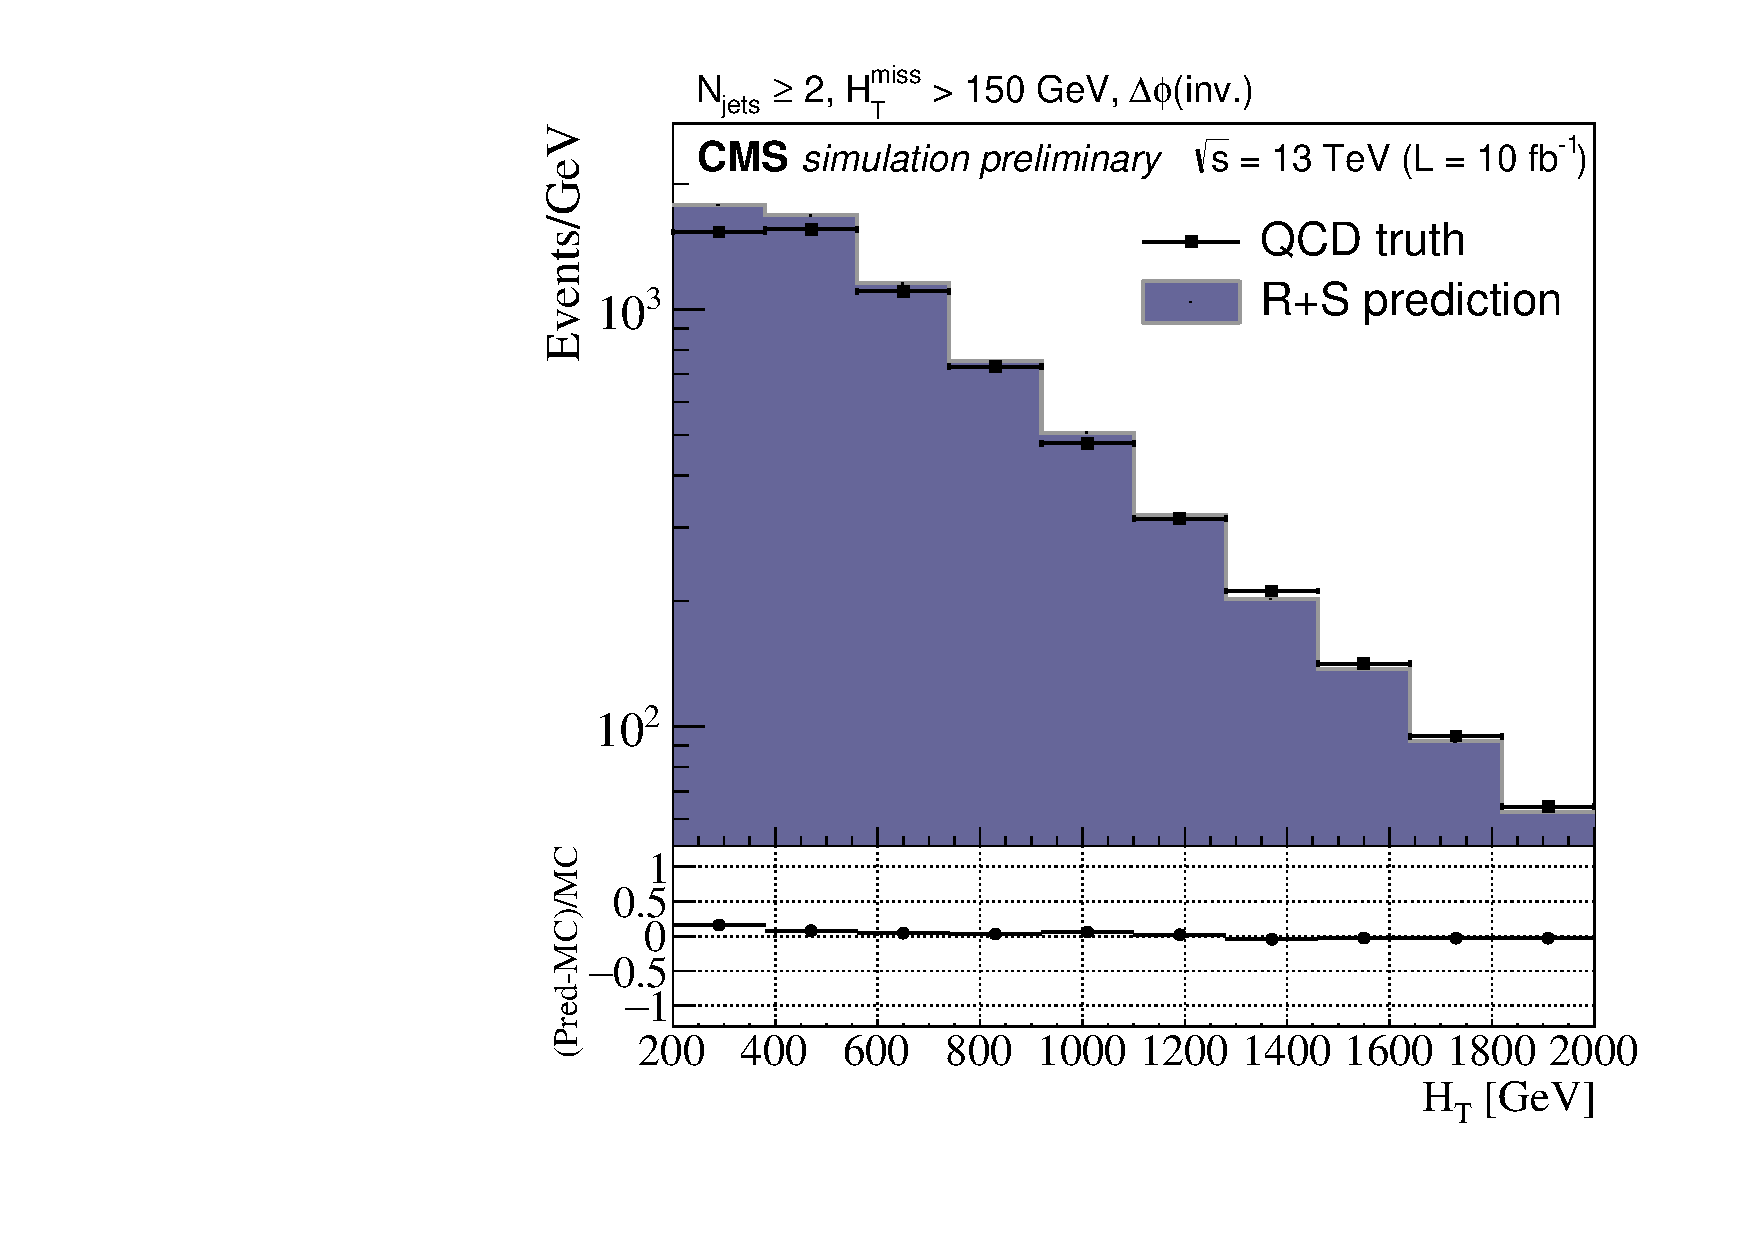
\includegraphics[width=0.5\linewidth]{figures/SusySearches/Ra2b2016/LowDeltaPhi_Ht.pdf}
}
\subfloat[]{
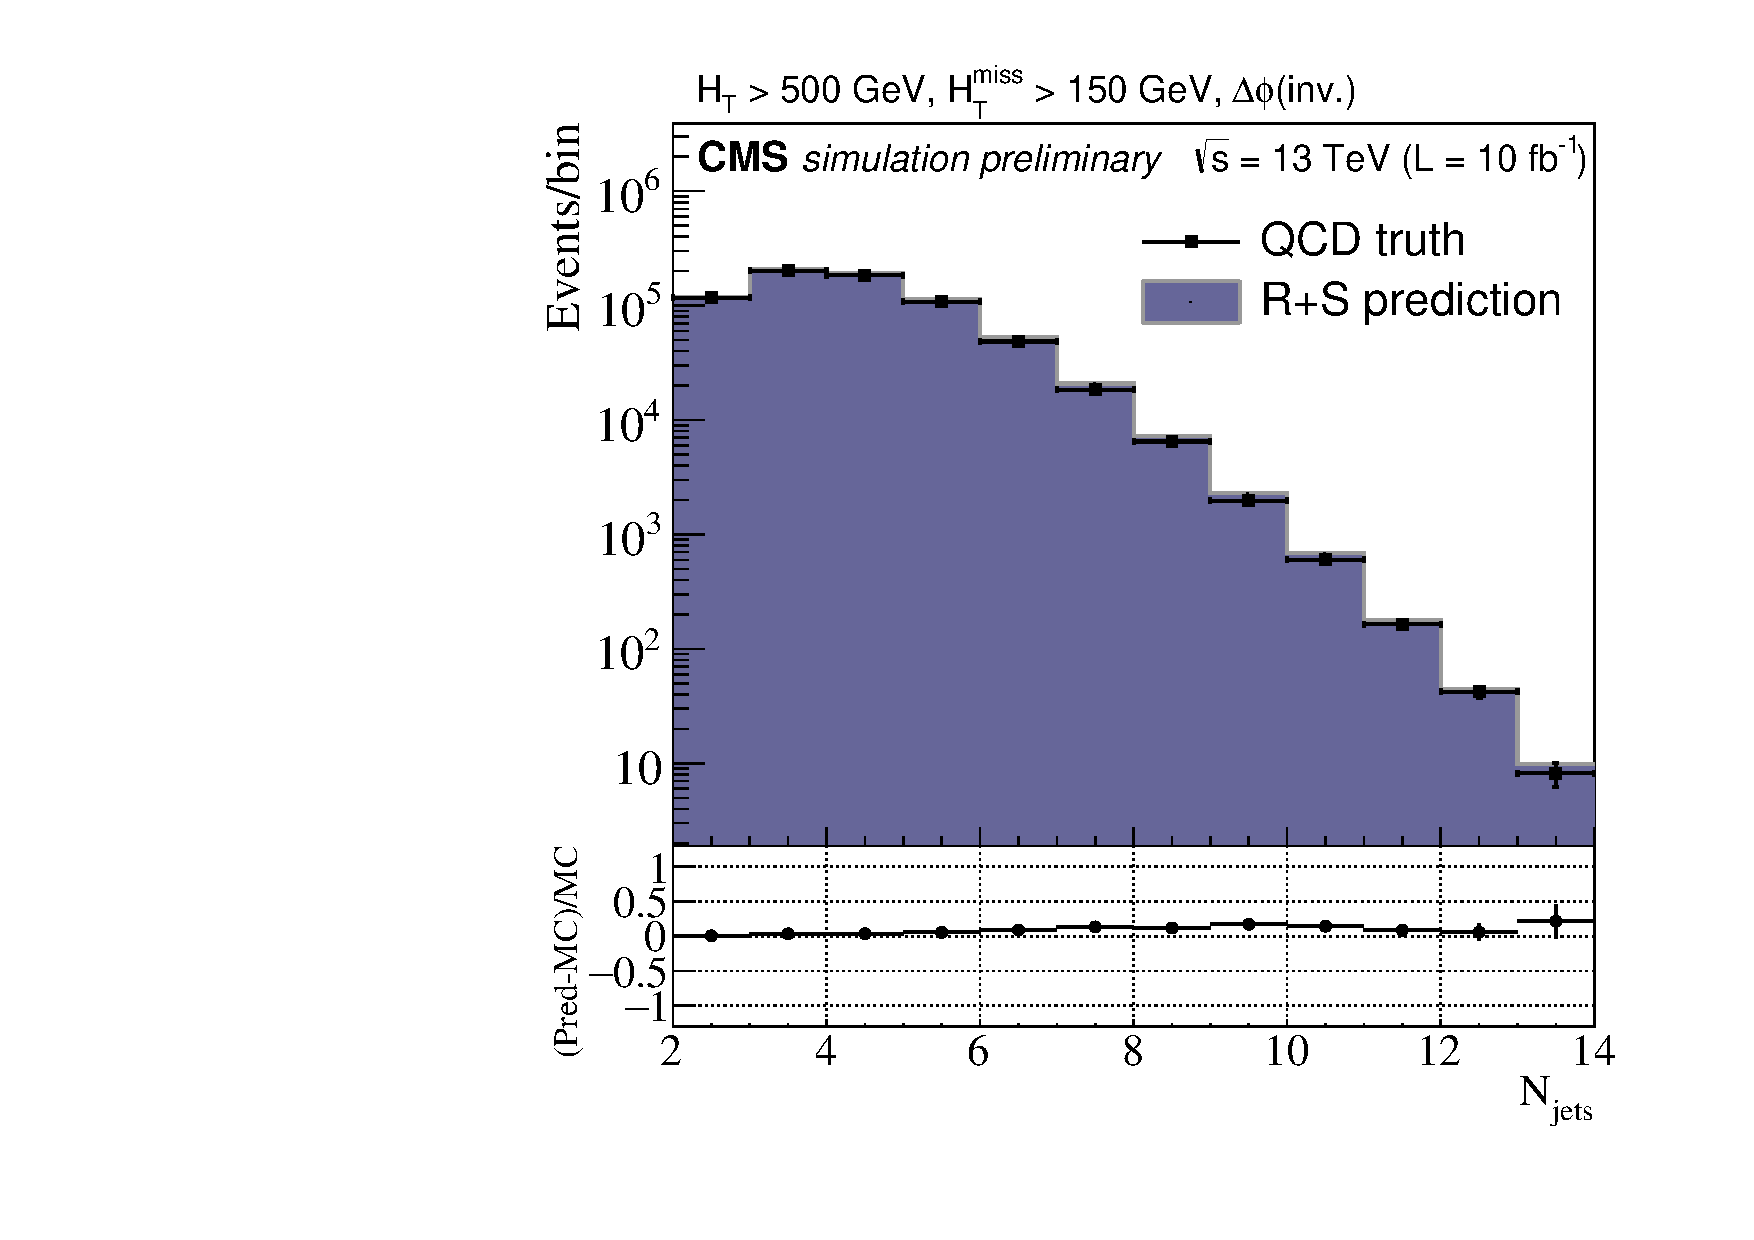
\includegraphics[width=0.5\linewidth]{figures/SusySearches/Ra2b2016/LowDeltaPhi_NJets.pdf}
}\\
\subfloat[]{
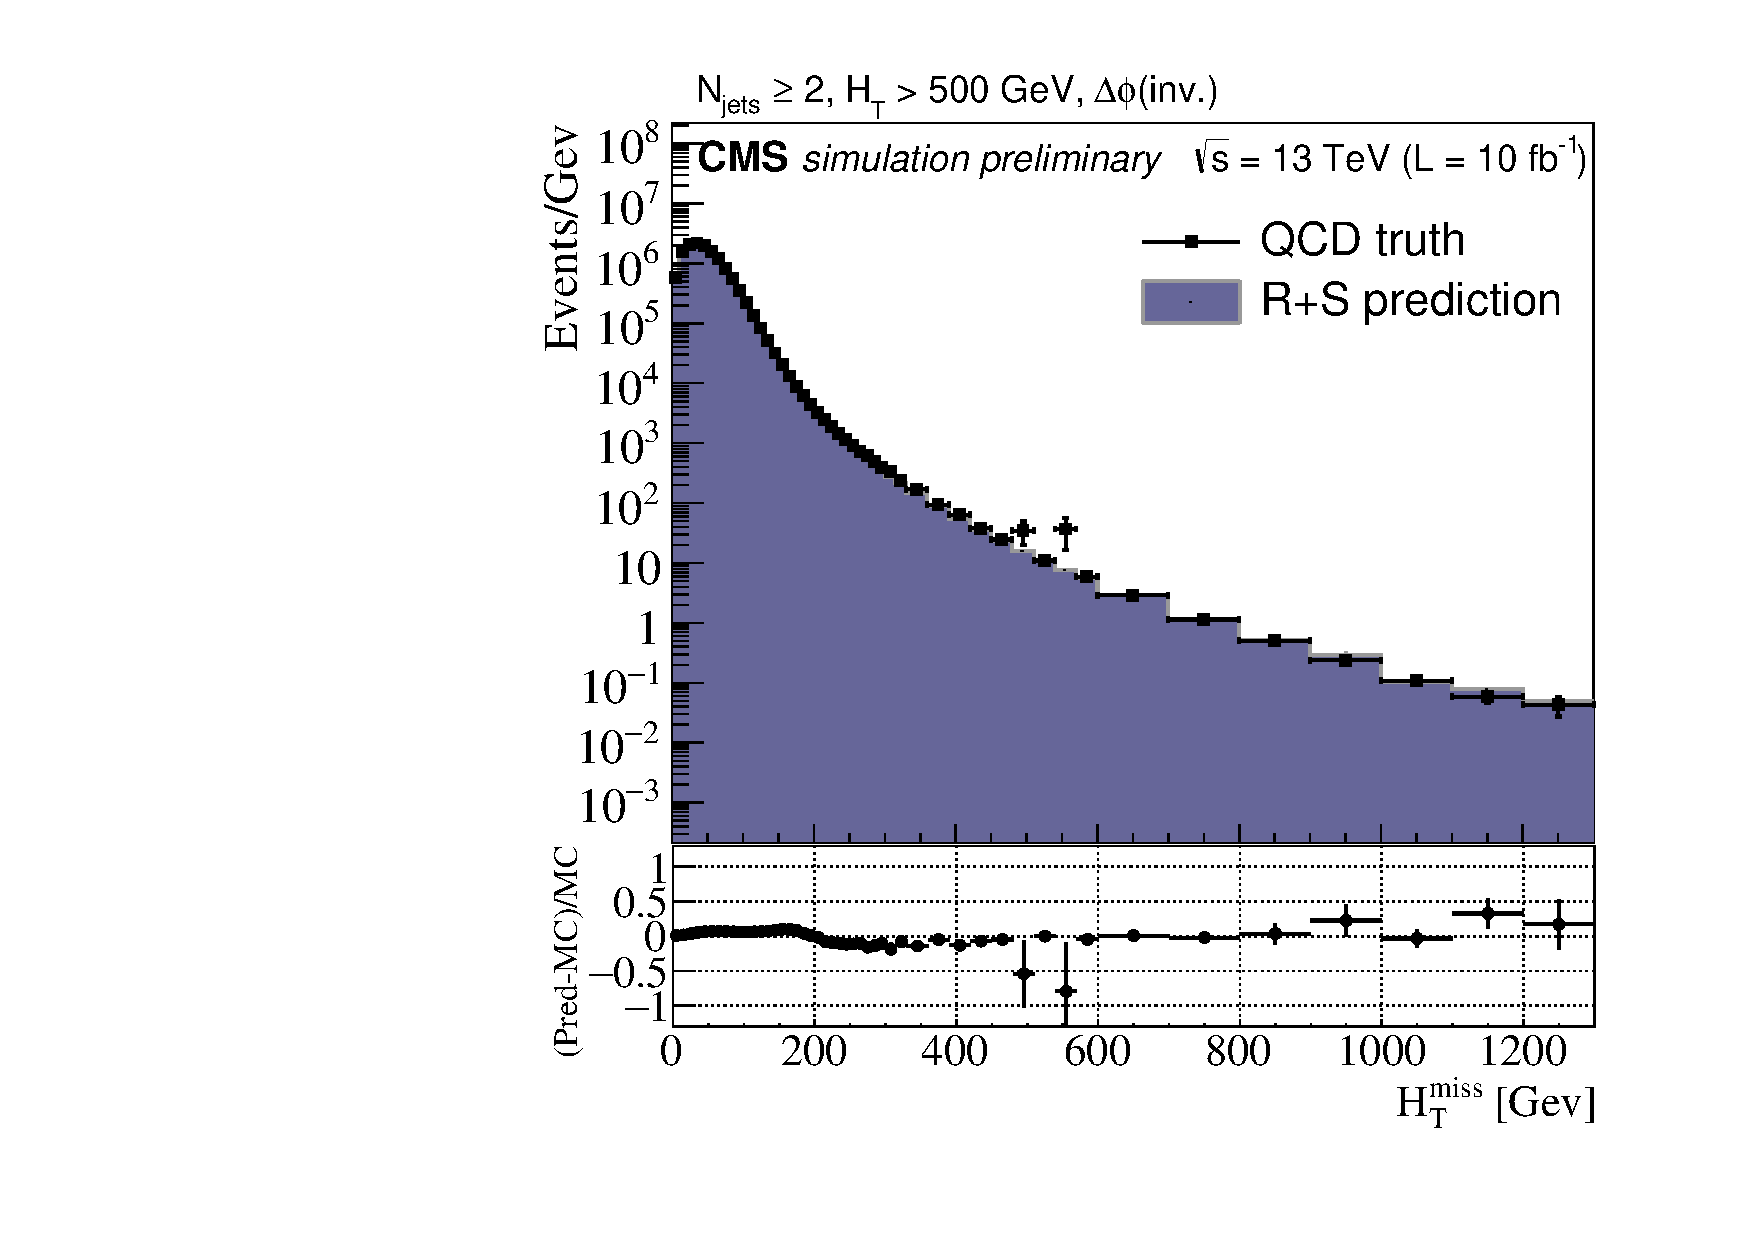
\includegraphics[width=0.5\linewidth]{figures/SusySearches/Ra2b2016/LowDeltaPhi_Mht.pdf}
}
\subfloat[]{
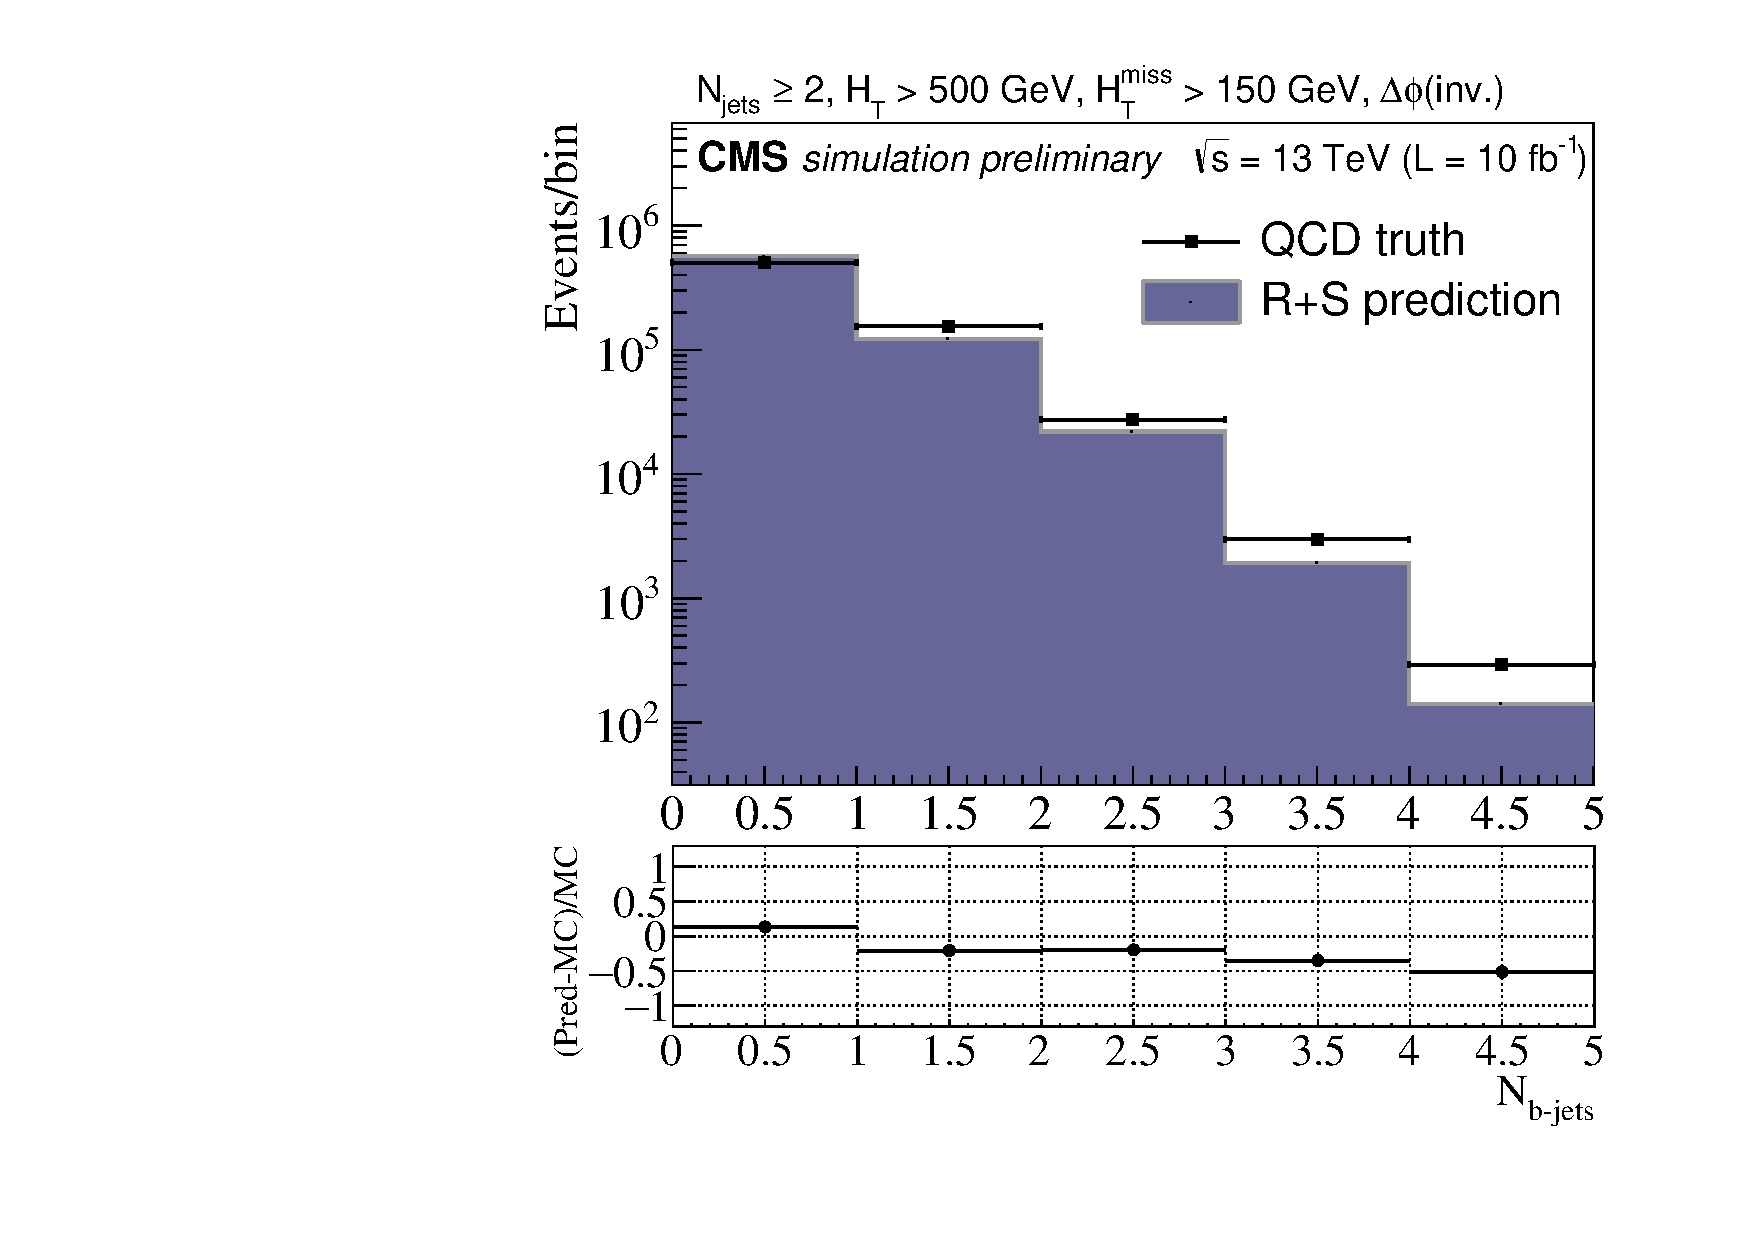
\includegraphics[width=0.5\linewidth]{figures/SusySearches/Ra2b2016/LowDeltaPhi_BTags.pdf}
}
\caption{Comparisons of kinematic distributions between the direct simulation and the rebalance and smear method applied to simulation, in the inverted $\Delta \phi$ control region of the multi-jet SUSY search.}
\label{fig:LowDeltaPhiRplusS}
\end{figure}


\begin{figure}[h]
\centering
\subfloat[]{
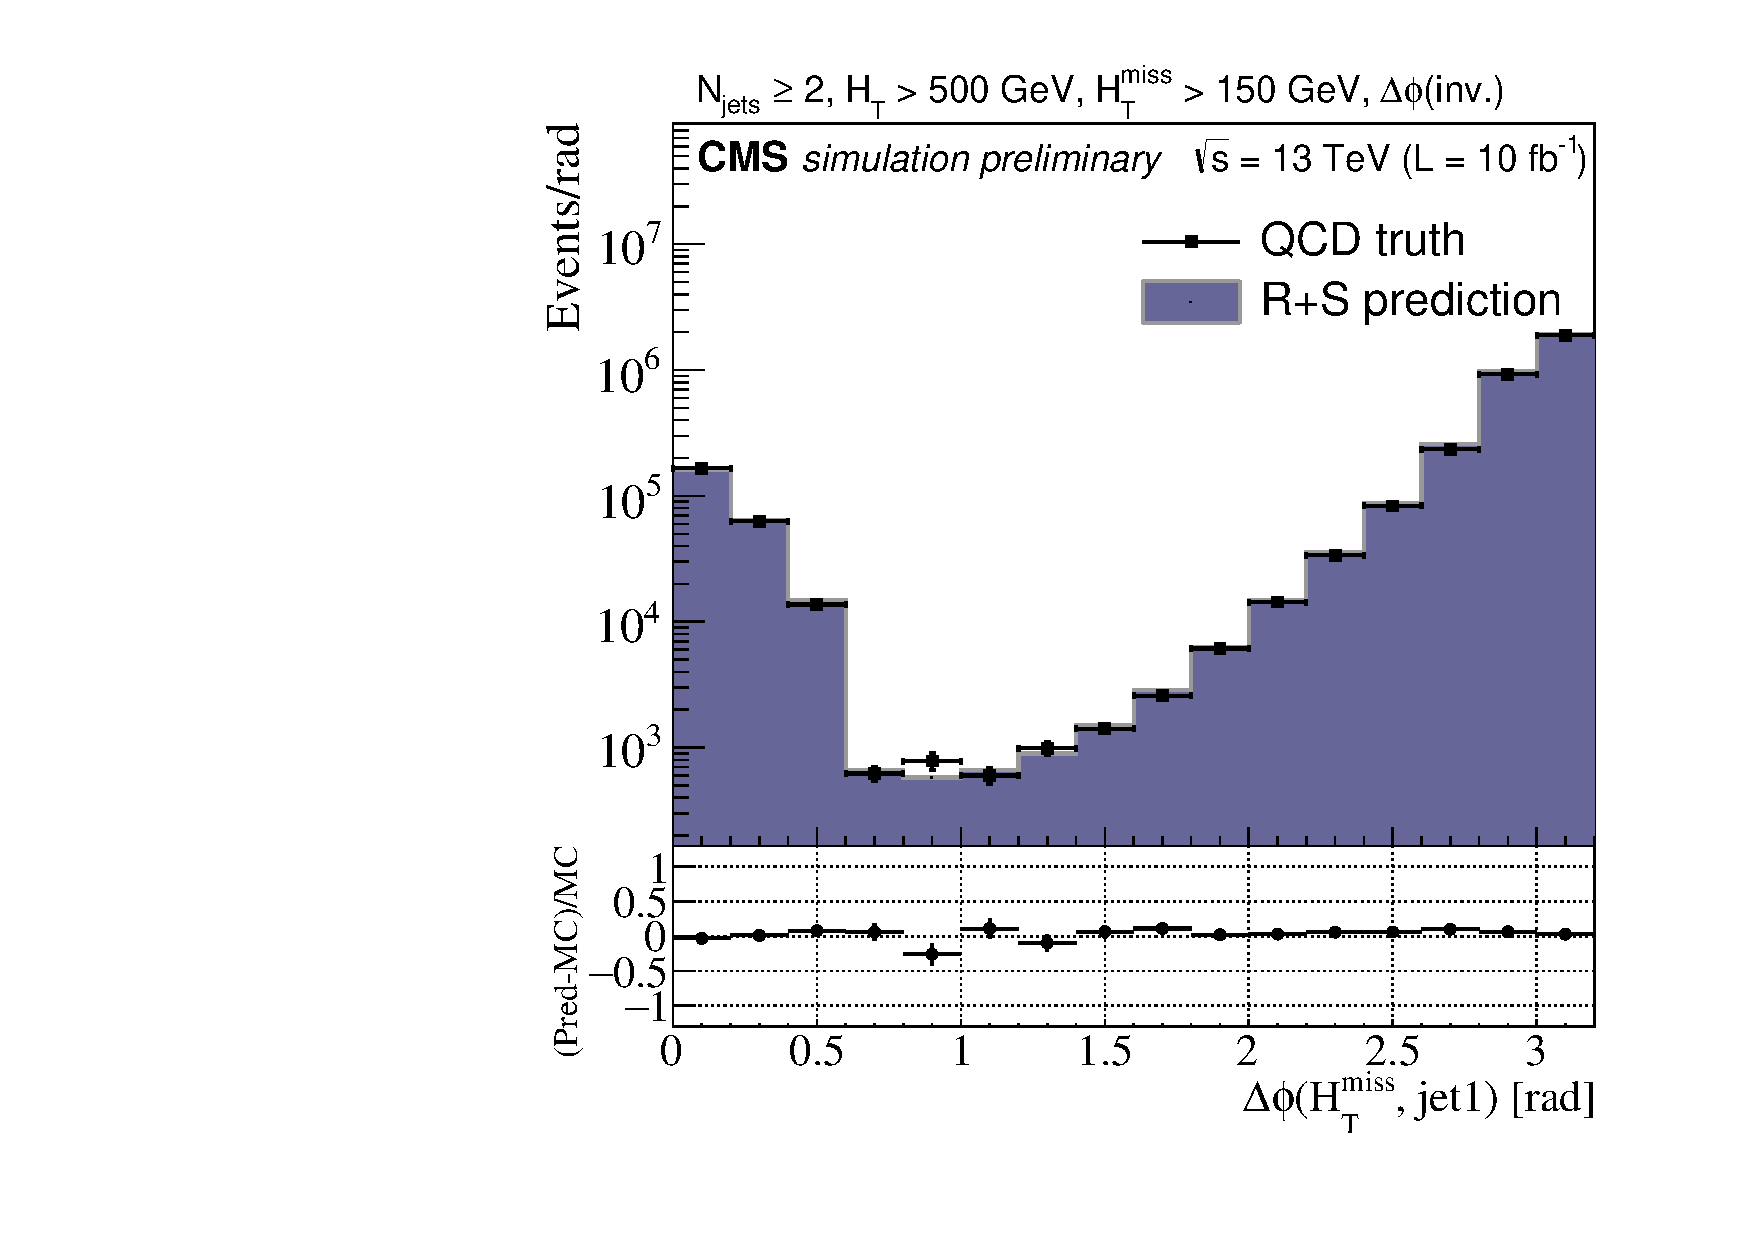
\includegraphics[width=0.5\linewidth]{figures/SusySearches/Ra2b2016/LowDeltaPhi_DPhi1.pdf}
}
\subfloat[]{
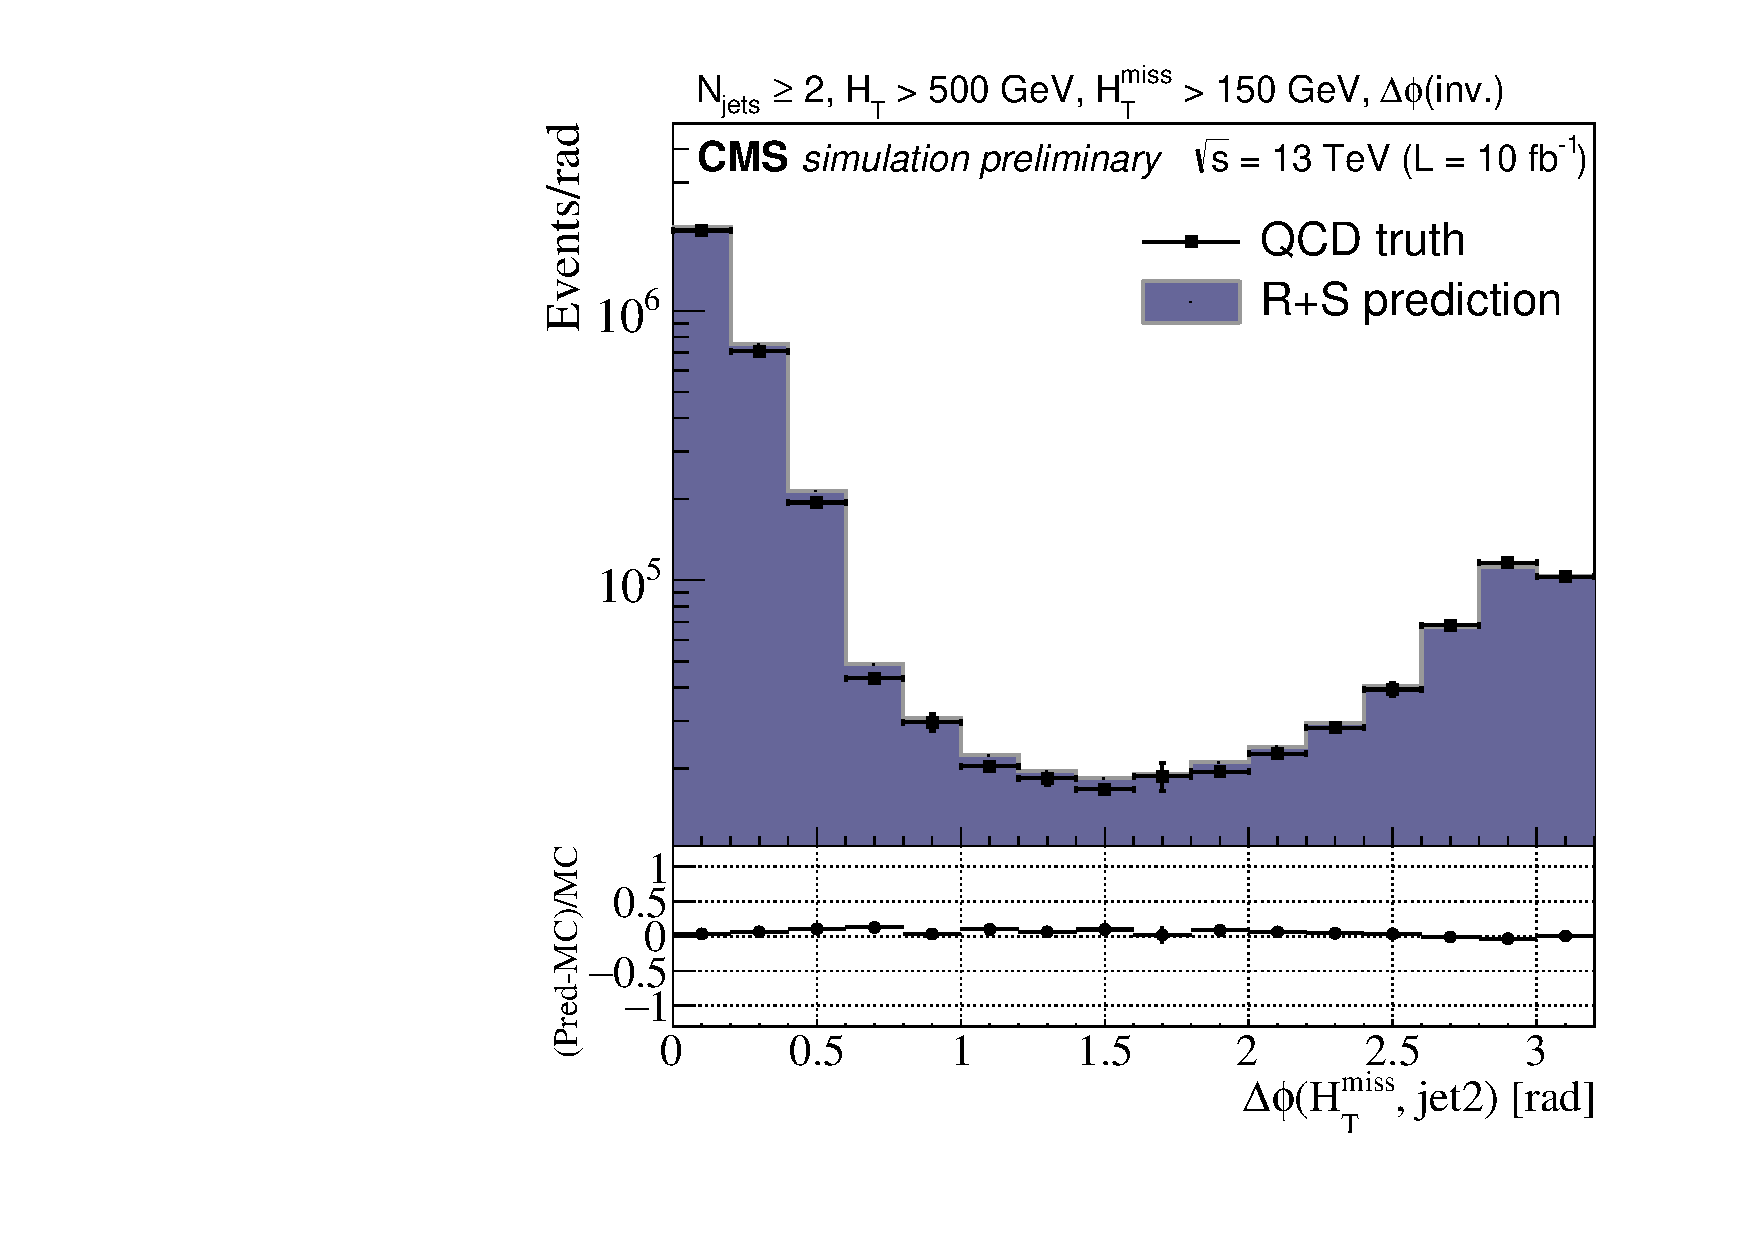
\includegraphics[width=0.5\linewidth]{figures/SusySearches/Ra2b2016/LowDeltaPhi_DPhi2.pdf}
}\\
\subfloat[]{
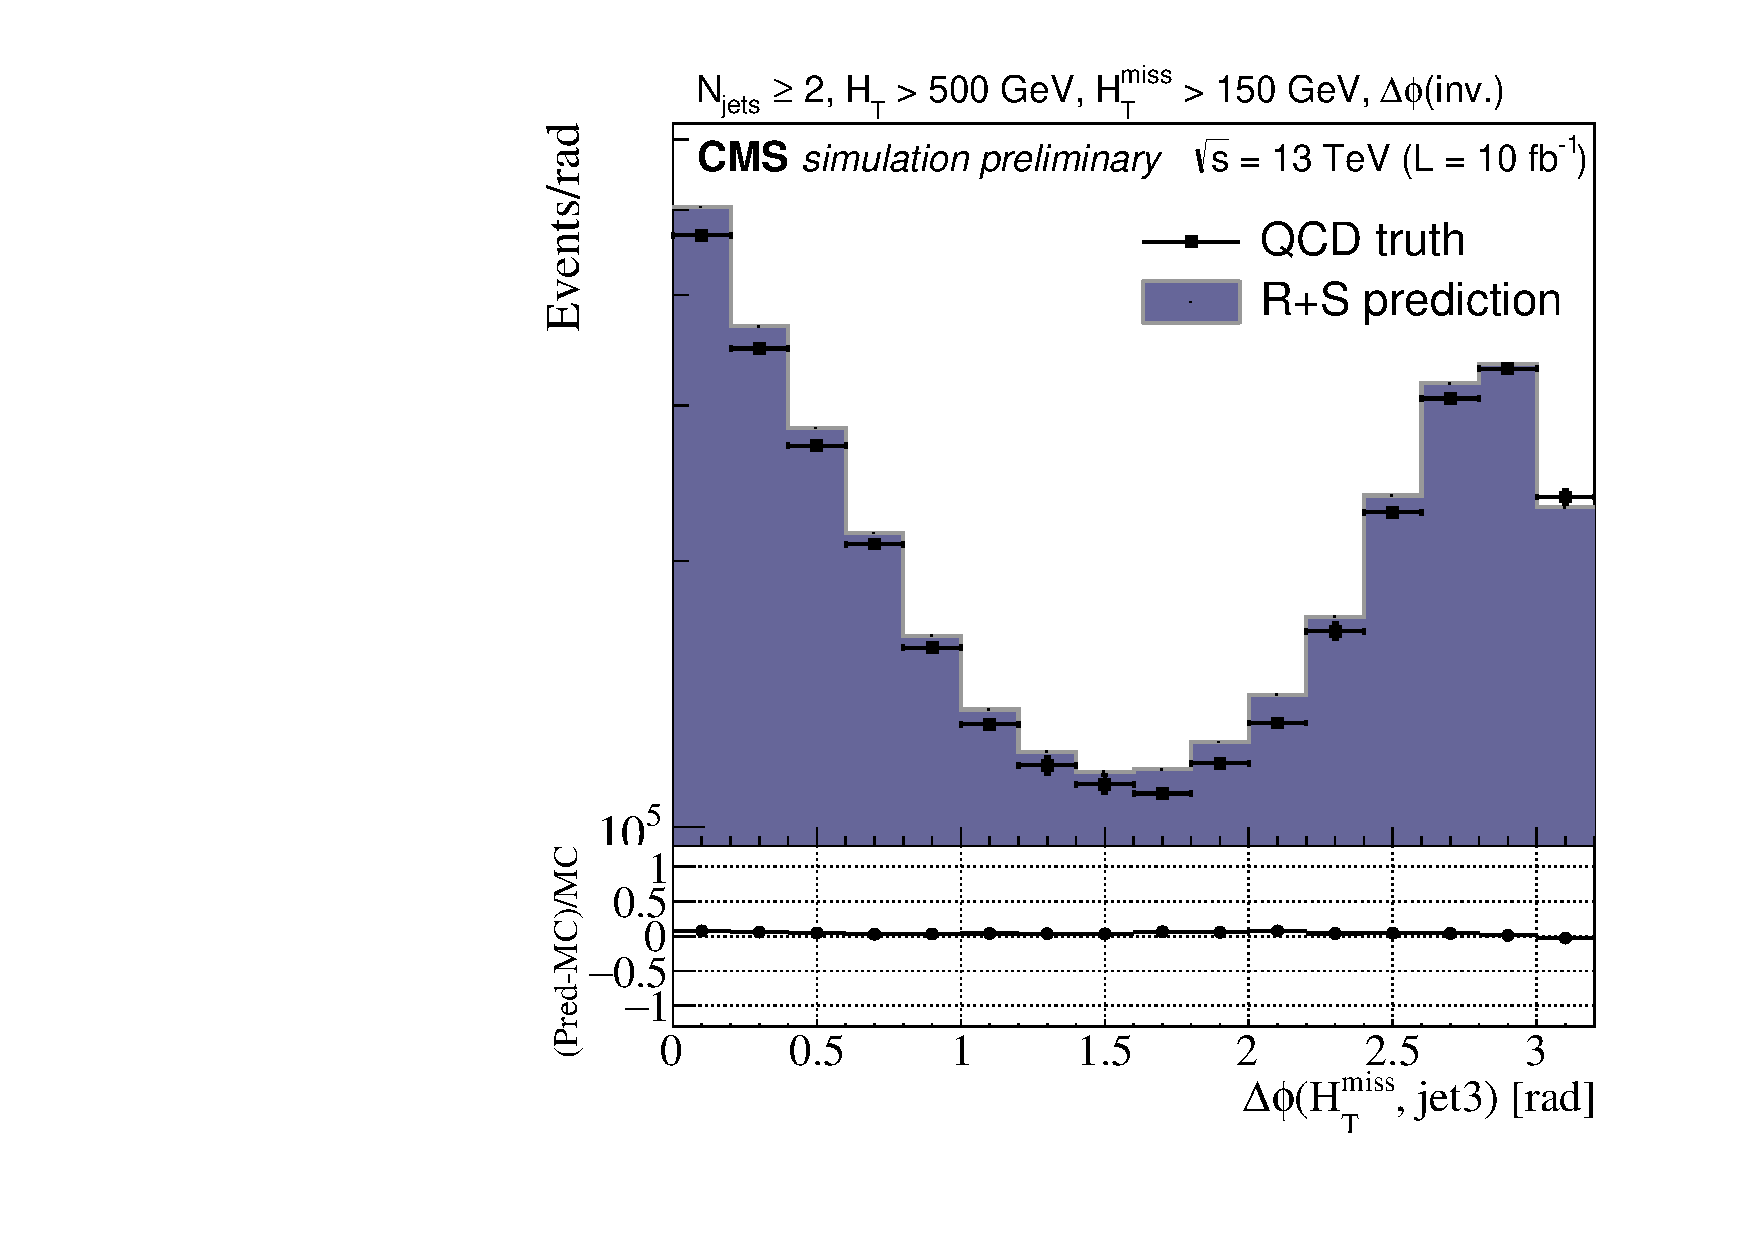
\includegraphics[width=0.5\linewidth]{figures/SusySearches/Ra2b2016/LowDeltaPhi_DPhi3.pdf}
}
\subfloat[]{
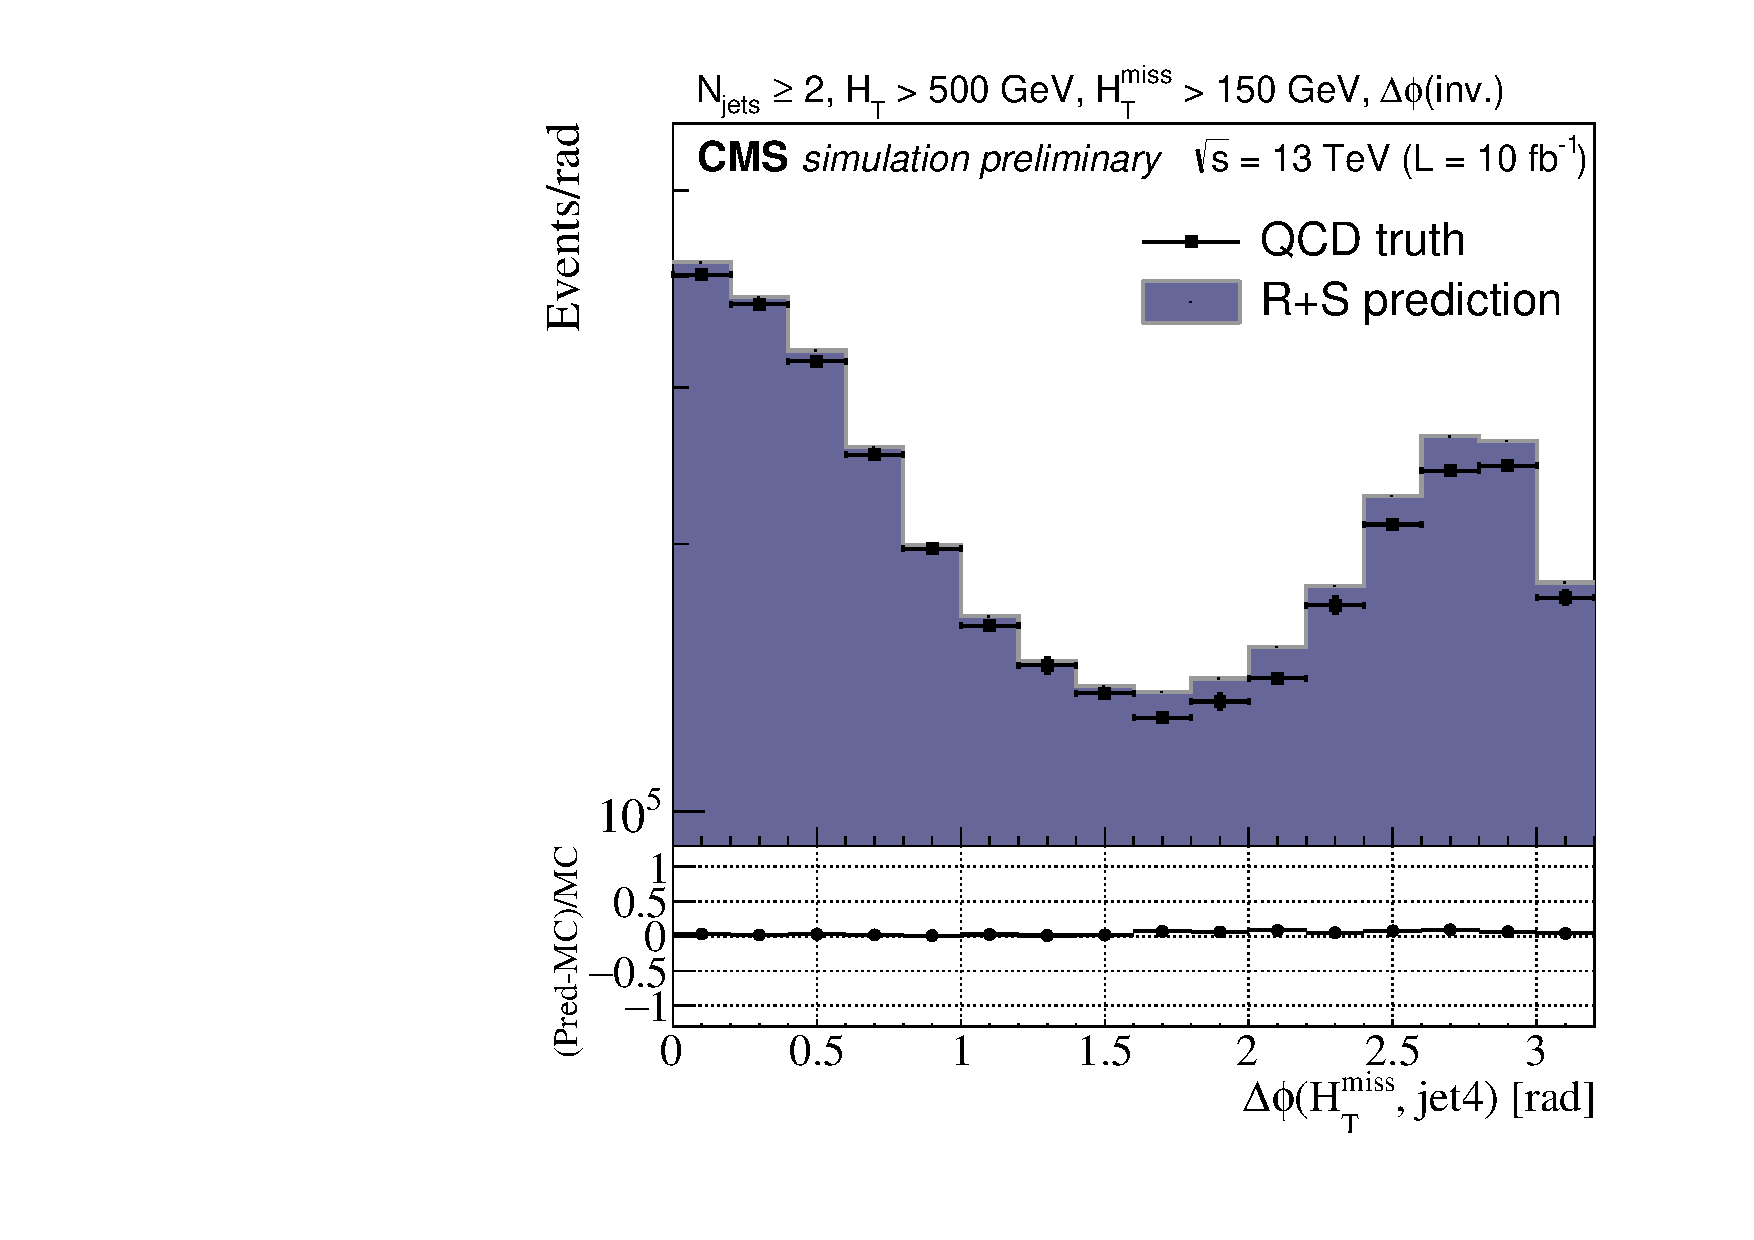
\includegraphics[width=0.5\linewidth]{figures/SusySearches/Ra2b2016/LowDeltaPhi_DPhi4.pdf}
}
\caption{Comparisons of kinematic distributions between the direct simulation and the rebalance and smear method applied to simulation, in the inverted $\Delta \phi$ control region of the multi-jet SUSY search.}
\label{fig:LowDeltaPhiRplusS2}
\end{figure}

\begin{figure}[h]
\centering
\subfloat[]{
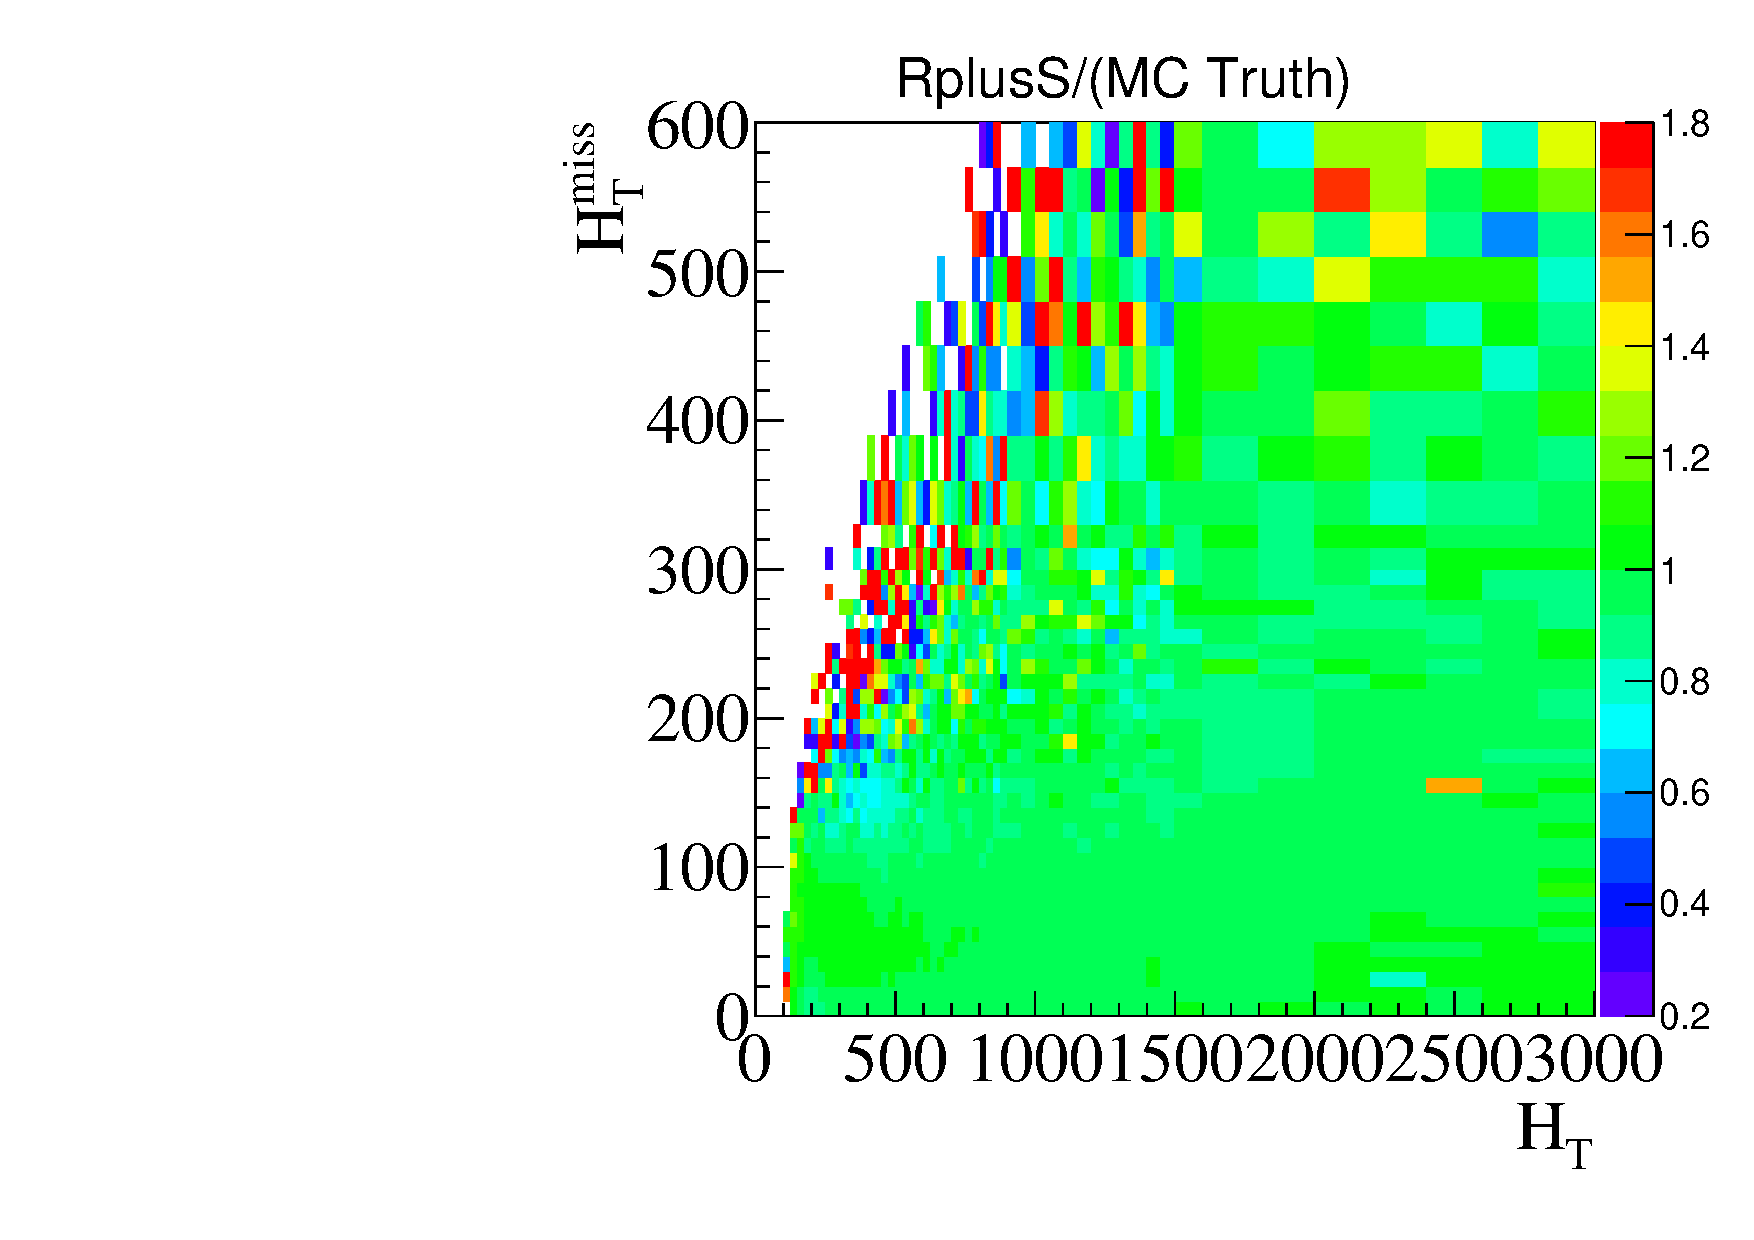
\includegraphics[width=0.5\linewidth]{figures/SusySearches/Ra2b2016/RplusSAndTruth_MhtVsHt.pdf}
}
\subfloat[]{
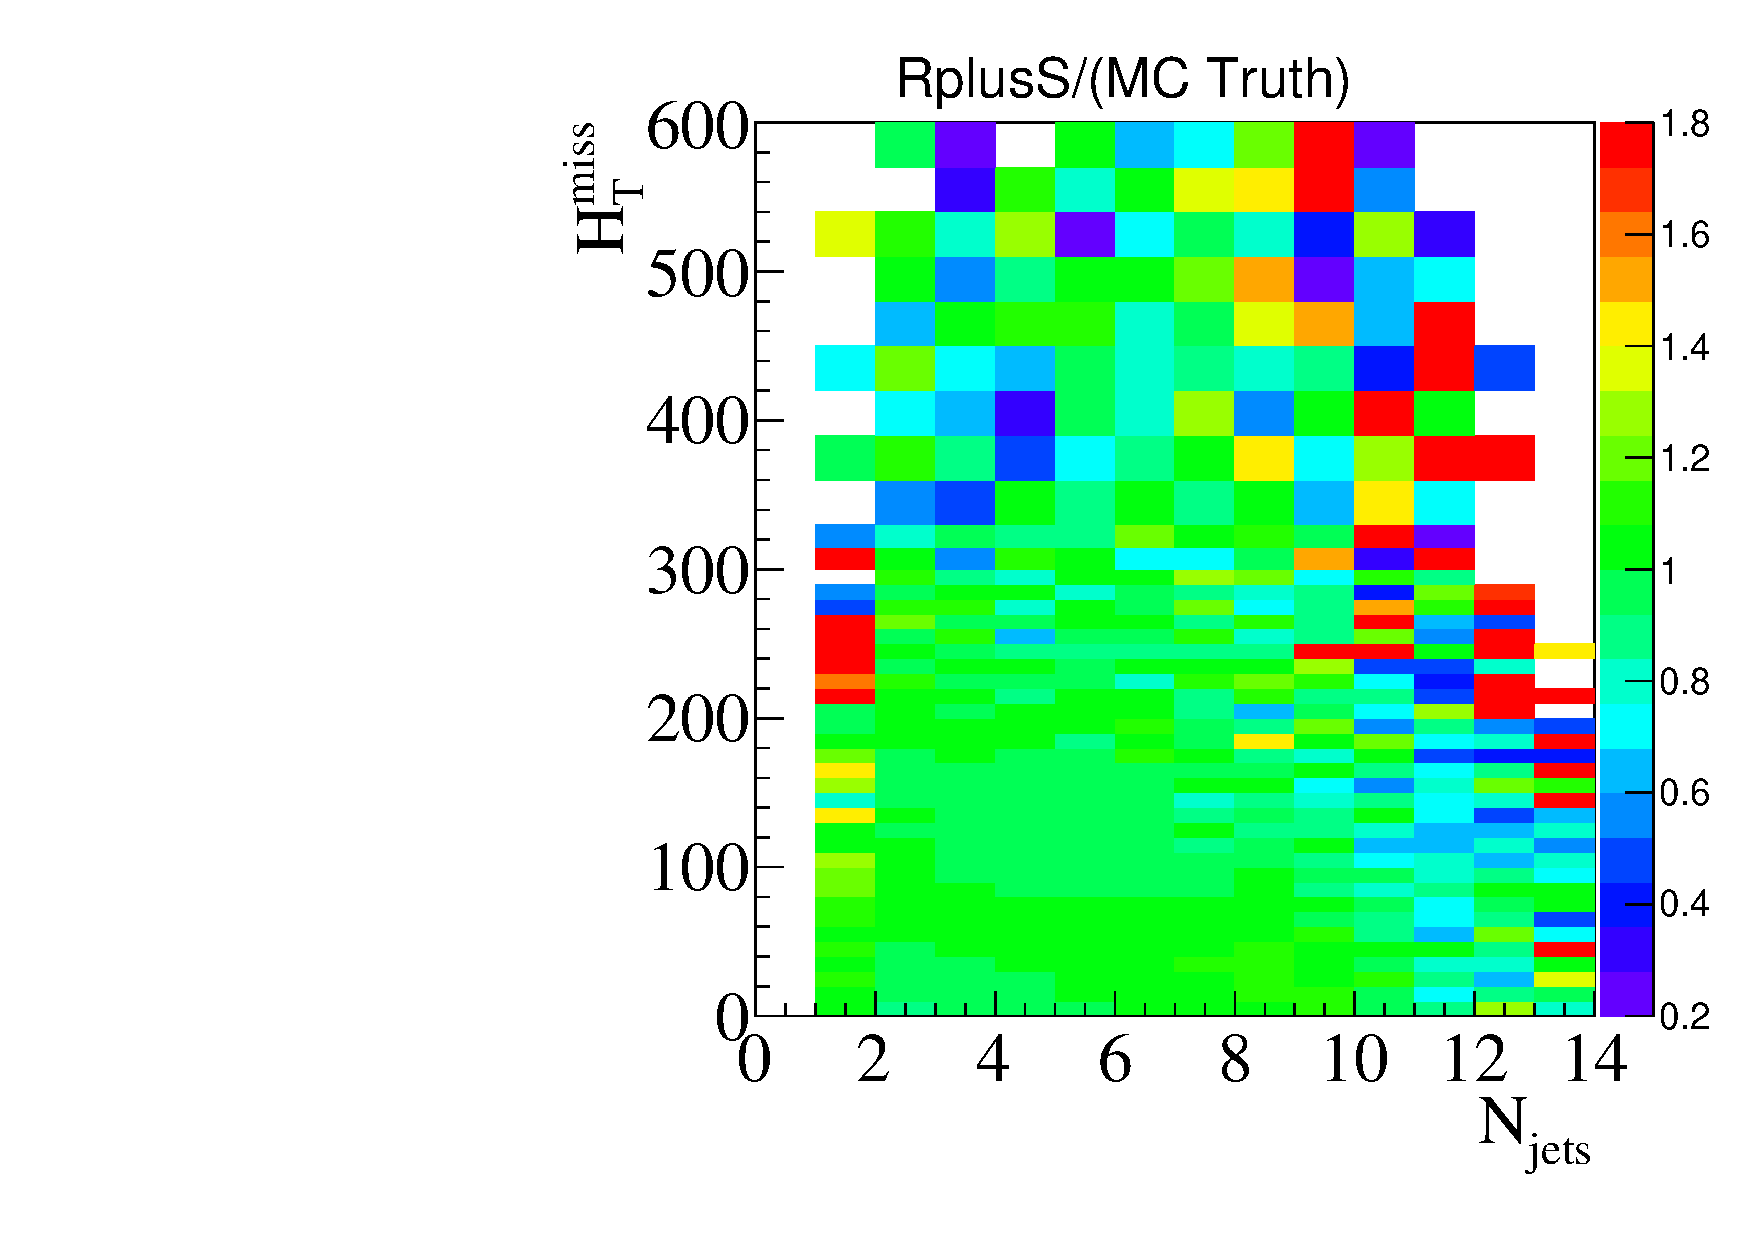
\includegraphics[width=0.5\linewidth]{figures/SusySearches/Ra2b2016/RplusSAndTruth_MhtVsNJets.pdf}
}\\
\subfloat[]{
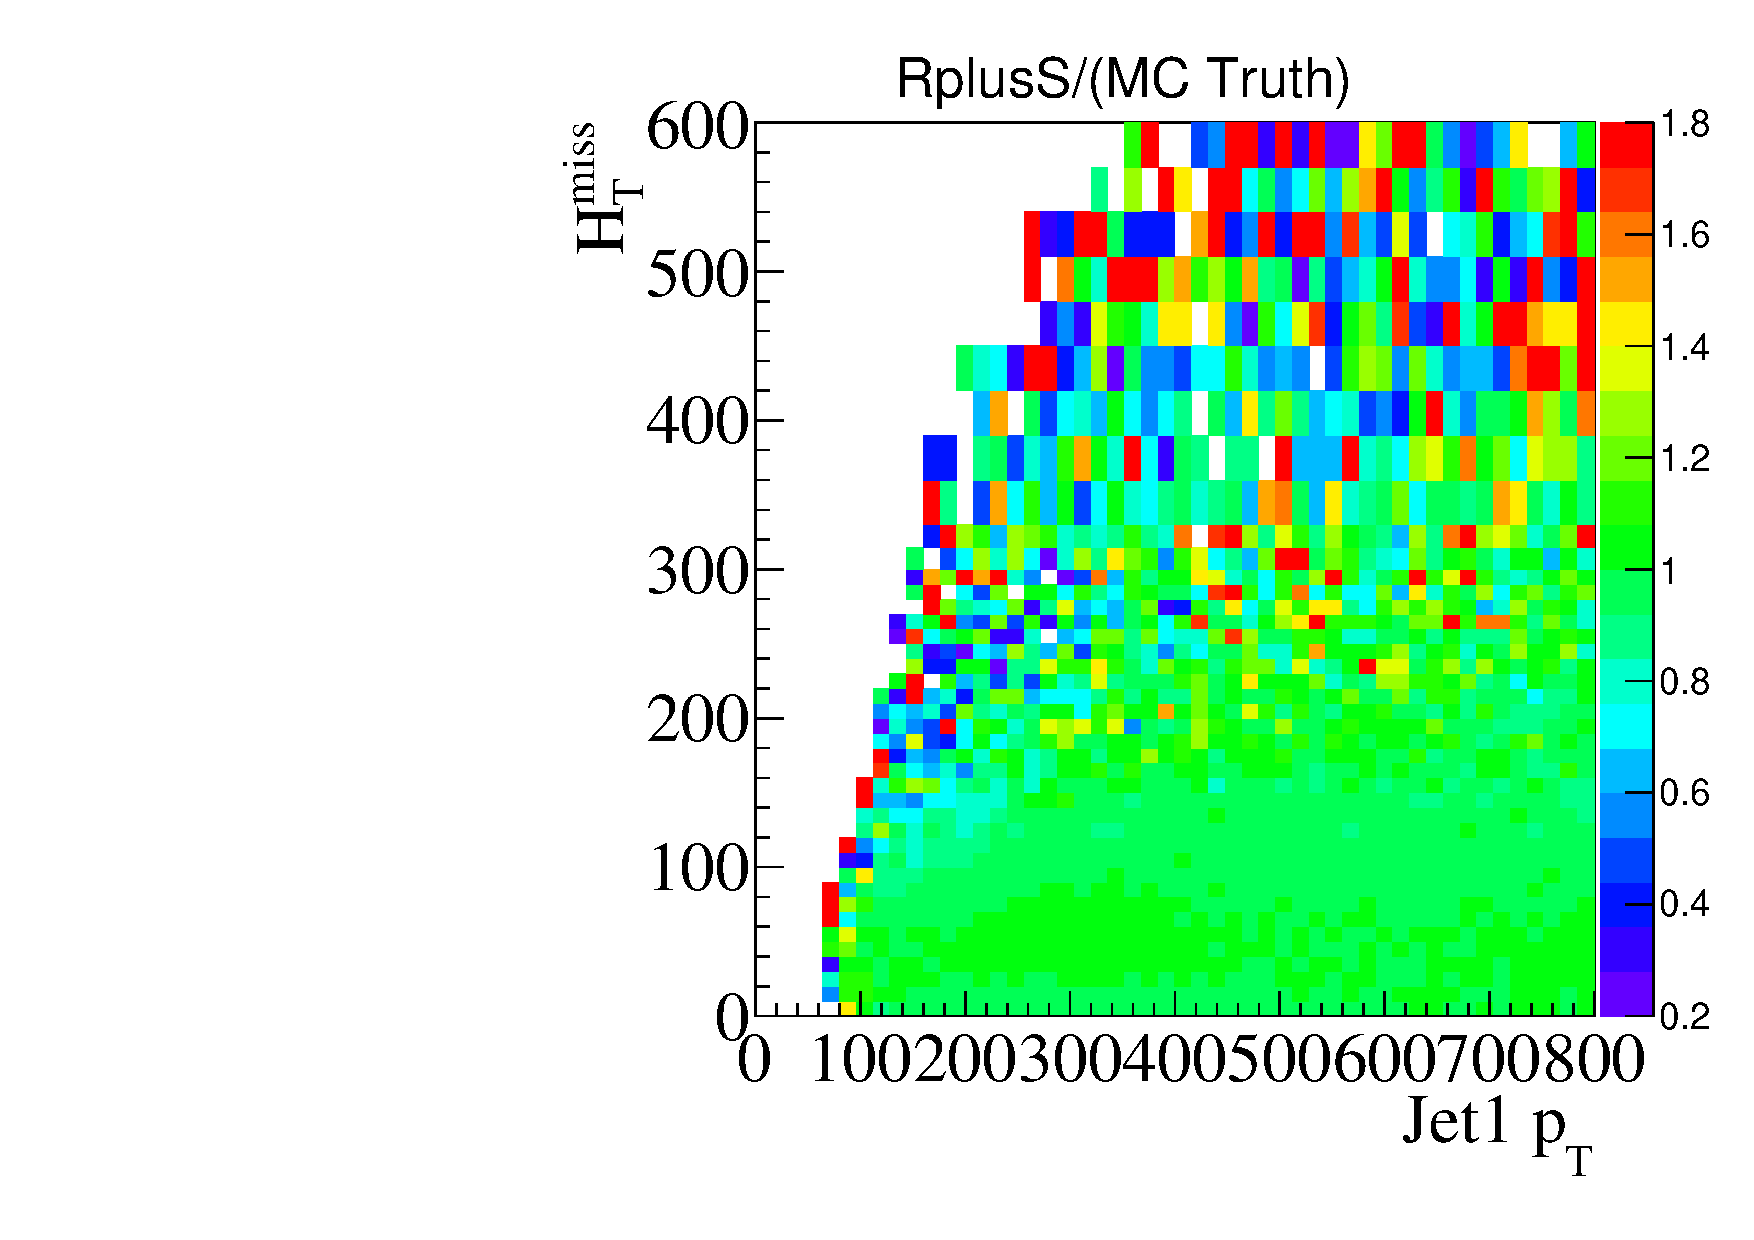
\includegraphics[width=0.5\linewidth]{figures/SusySearches/Ra2b2016/RplusSAndTruth_MhtVsJet1Pt.pdf}
}
\subfloat[]{
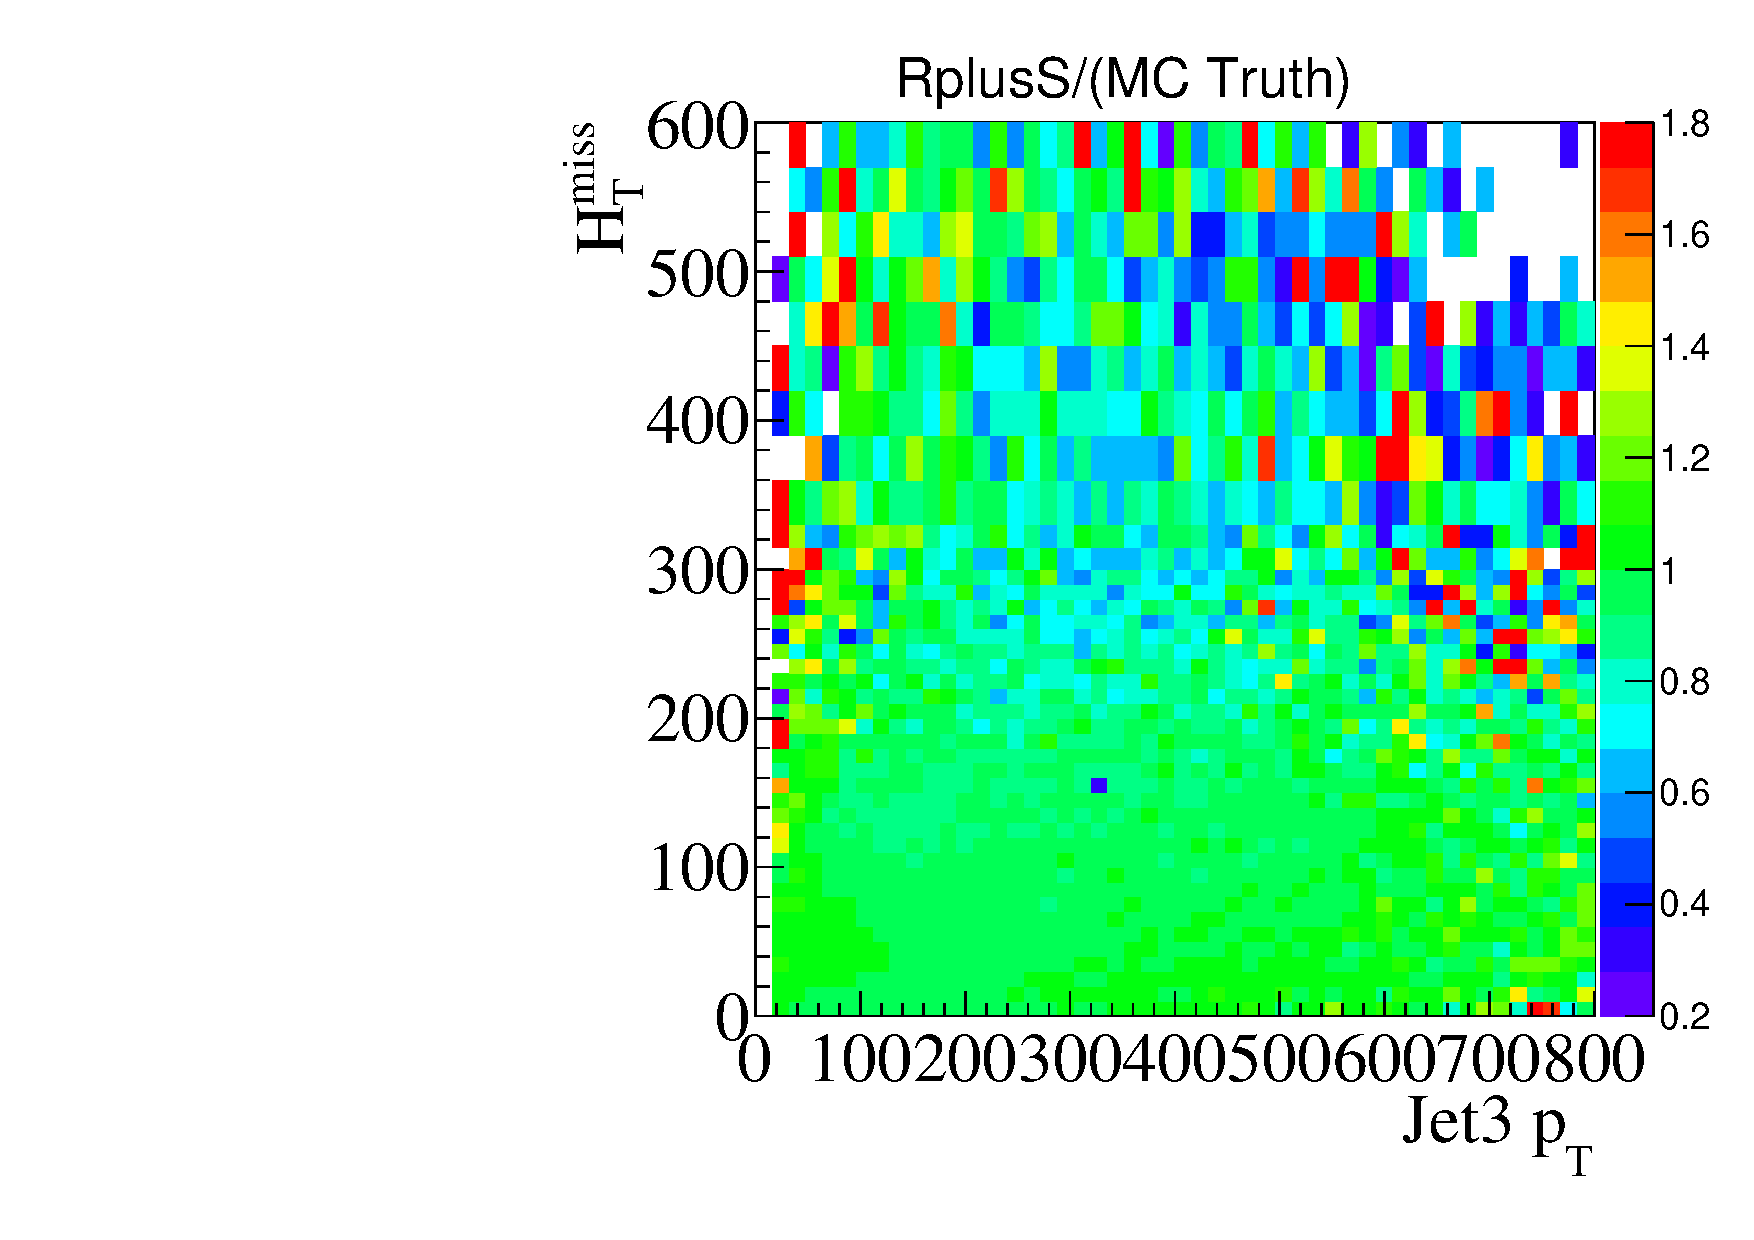
\includegraphics[width=0.5\linewidth]{figures/SusySearches/Ra2b2016/RplusSAndTruth_MhtVsJet3Pt.pdf}
}
\caption{The ratio of scatter plots of key observables for hadronic SUSY searches between the direct simulation and the rebalance and smear method applied to simulation.}
\label{fig:RplusSCorrelation}
\end{figure}
\FloatBarrier
\noindent
The degree of consistency between the prediction and expectation is excellent in all considered kinematic regions, with the exception of large $\nbjets$ region. Not only are the relevant 1-dimensional distributions accurately modeled, but all pairwise correlations of the kinematic observables examined show good closure. This includes correlations between the directions and magnitudes of the momenta of jets within an event, as well as relationships between the directions of the $\mht$ and the jets, and the magnitudes of the $\mht$ and $\Ht$. The most significant exception to these statements is with the distribution of the multiplicity of b-tagged jets,  where non-closure is evident for events with $\geq 3$ b-jets on the order $\approx50\%$. A possible source of this discrepancy is the choice of binning for the parton-level $\mht$ templates that constitute the prior, namely, $\nbjets=$ 0, 1, and $\geq$ 2.  A modification of this choice to include templates for the individual bins of $\nbjets=$ 2, 3, and $\geq 4$ may lead to improved results in the region of large b-jet multiplicity. 

The method is ready to be applied in the data, but I first give a summary of the key developments, a note on the strengths of the method, and a breakdown of uncertainties associated with the method.

\subsubsection{What were the key developments?}
It appears to be feasible to use correlations among jets in QCD events as a means of achieving signal-background discrimination in kinematic regions dominated by QCD, such as the regions of low-$\mht$ and low $\Ht$. The possibility of applying the method in the low-$\mht$ region is for the first time feasible. It was not possible before because the classical method does not accurately model the QCD kinematics in this region (see Fig. \ref{fig:OldVsNew}). 
\begin{figure}[h]
\centering
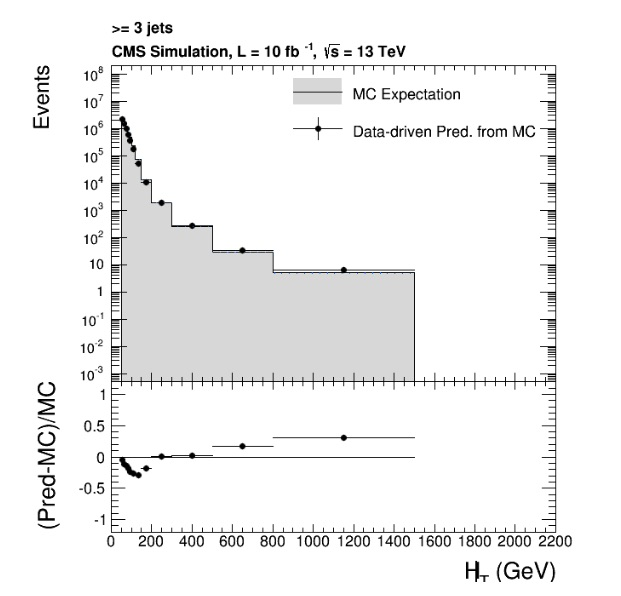
\includegraphics[width=0.49\linewidth]{figures/SusySearches/Ra2b2016/RnSClassicMht.jpg}
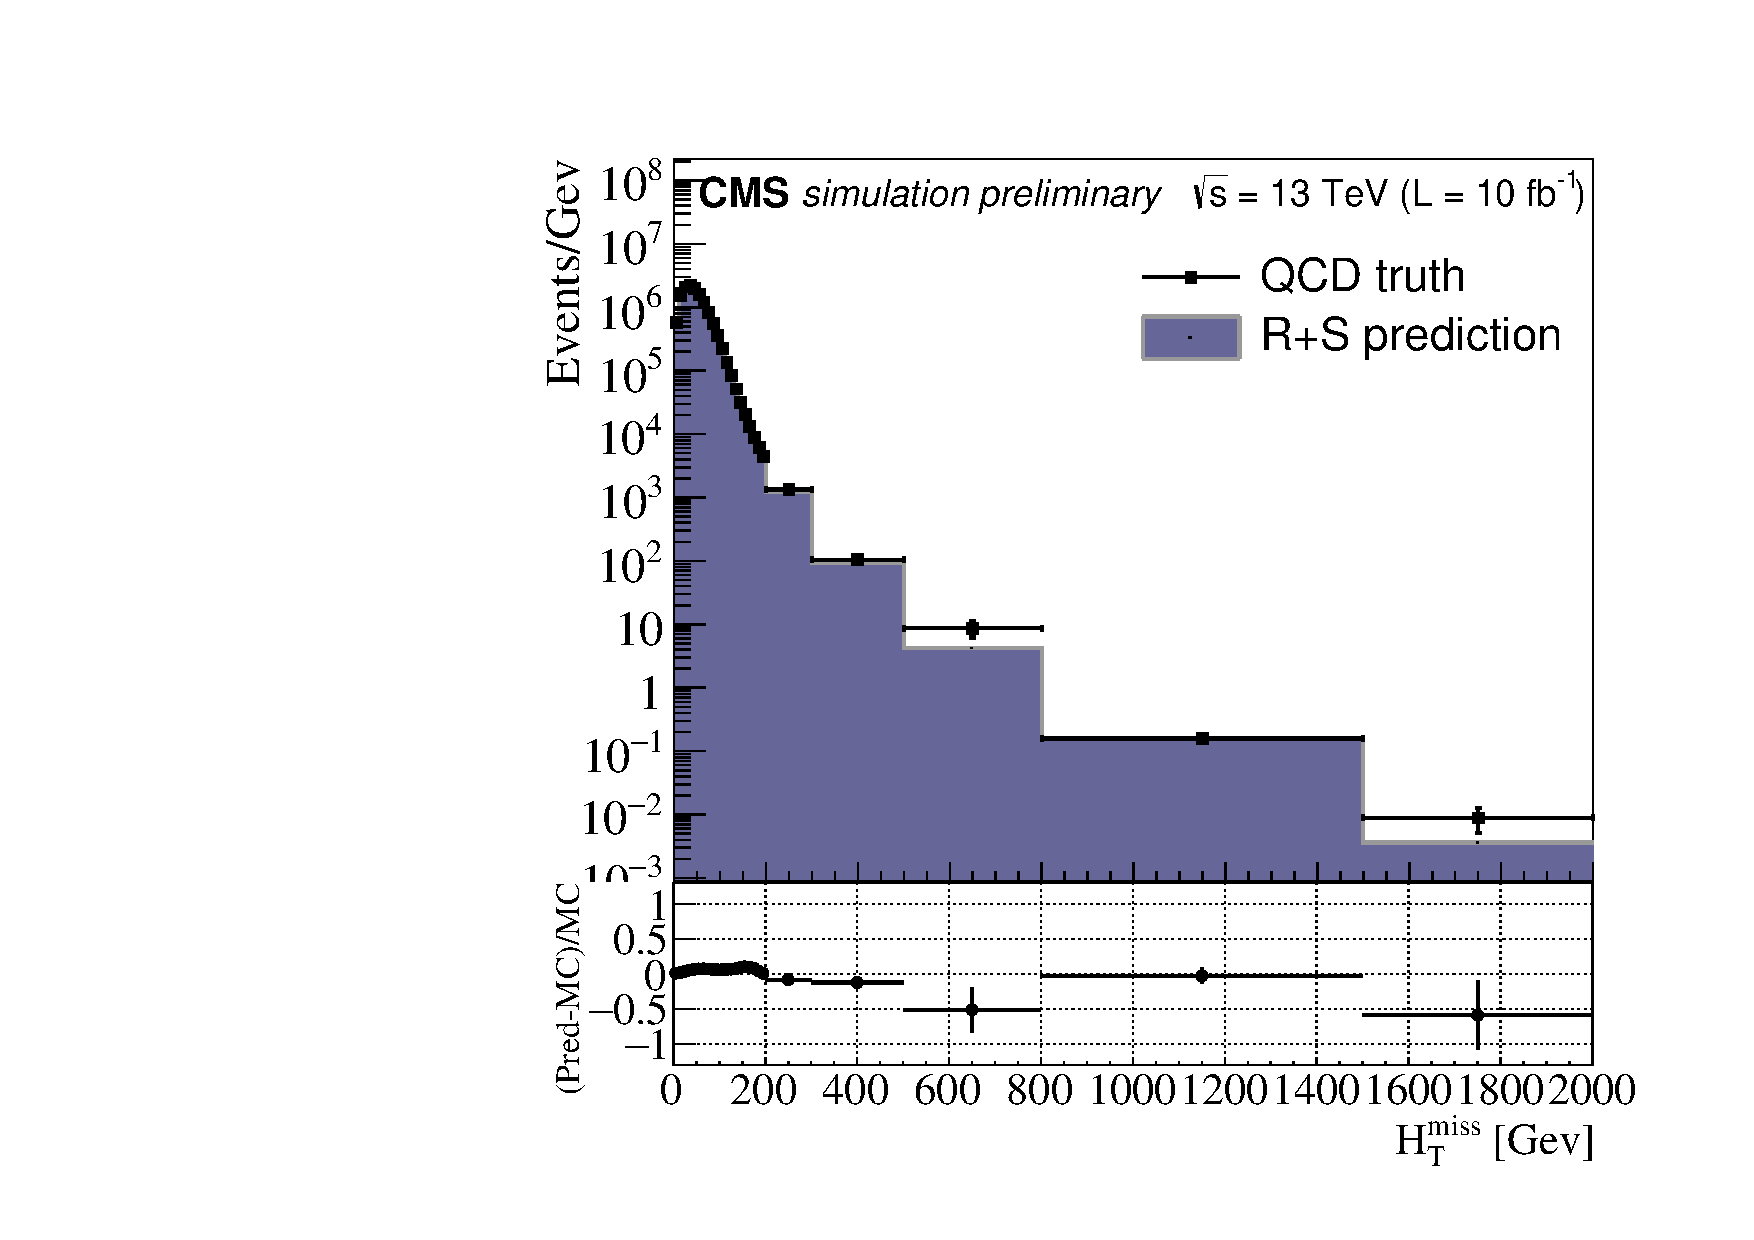
\includegraphics[width=0.49\linewidth]{figures/SusySearches/Ra2b2016/LowDeltaPhi_MhtForComparison.pdf}
\caption{Comparisons of the $\mht$ distribution between prediction and expectation using the classical method (left) and the new method (right).}
\label{fig:OldVsNew}
\end{figure}
The primary reasons for these improvements with respect to the classical method are that a realistic parton-level $\mht$ constraint is used in the rebalance procedure, whereas, in the classical method, every event is rebalanced to an $\mht$ of 0 or a constant value chosen by the user, amounting to a delta function constraint. Second, the full jet response has been used in the likelihood maximization, rather than gaussian approximations. Gaussian approximations can lead to mis-modeling of the jet $\pt$ or $\mht$ spectrum in events containing jets with small $\pt$, which exhibit a highly non-Gaussian response. 

The rebalance and smear method is robust against contamination from signal events in the prediction sample. The reason is that the rebalance procedure displaces signal-like, high-$\met$ events from the high-$\met$ region, to regions of low-$\met$; after smearing, the proportion of events in the high-$\met$ region truly originating from QCD processes is nearly 100\% (see Fig. \ref{fig:RplusSContamination}). 
\begin{figure}[tb!]
\centering
\includegraphics[width=0.6\linewidth]{figures/SusySearches/Ra2b2016/RplusSContam.pdf}
\caption{Signal contaimination removal. The midnight blue (and yellow) histograms show the distribution of QCD (and signal) events taken directly from simulation. The black (and red) histograms show the distributions of QCD (and signal) and after being processed by the rebalance and smear procedure. The signal has been removed from the high-$\mht$ region, leaving an accurately modeled QCD contribution.}
\label{fig:RplusSContamination}
\end{figure}
The robustness of the prediction to possible signal contamination in the control region allows for real events to be used directly for the prediction. Another strength is that the rebalanced events can be smeared an indefinite number of times, which allows for the accumulation of an indefinitely large prediction sample, computer resources permitting. Therefore, estimates of the expected QCD event count and uncertainty are made in extreme tails, even in regions for which no simulated QCD events are available, or for which the expected count is much less than 1. Alternatively, the rebalanced events can smeared once to generate a training sample of background events for a multivariate discriminant, and subsequent smearing can generate a statistically-independent prediction sample. This is further explored in Chapter \ref{chap:money}. Essentially, this approach establishes a data-driven QCD event generator.
\FloatBarrier

\subsection{Applying the method in data}
To derive the rebalance and smear prediction using real data, samples are collected with a series of pre-scaled $\Ht$ triggers,
\begin{itemize}
  \item \texttt{HLT\_PFHT200\_*},
    \item \texttt{HLT\_PFHT300\_*},
      \item \texttt{HLT\_PFHT350\_*},
        \item \texttt{HLT\_PFHT600\_*},
\end{itemize}
and the un-prescaled trigger,
\begin{itemize}
  \item \texttt{HLT\_PFHT800\_*}.
\end{itemize}
Events collected by these triggers are pooled into a single sample, here referred to as the $\Ht$ control sample. Events are rejected if the trigger with the highest possible $\Ht$ threshold that could have fired did not fire. This criterion ensures that the probability of an event being selected is equal to the the inverse of the pre-scale, since events with large $\Ht$ that happen to trigger one of the lower $\Ht$ triggers would otherwise inflate the probability slightly. Distributions of the weighted and un-weighted online $\Ht$, and un-weighted offline $\Ht$ are shown in Fig. \ref{fig:PrescaleWeights}.
\begin{figure}[tb!]
\centering
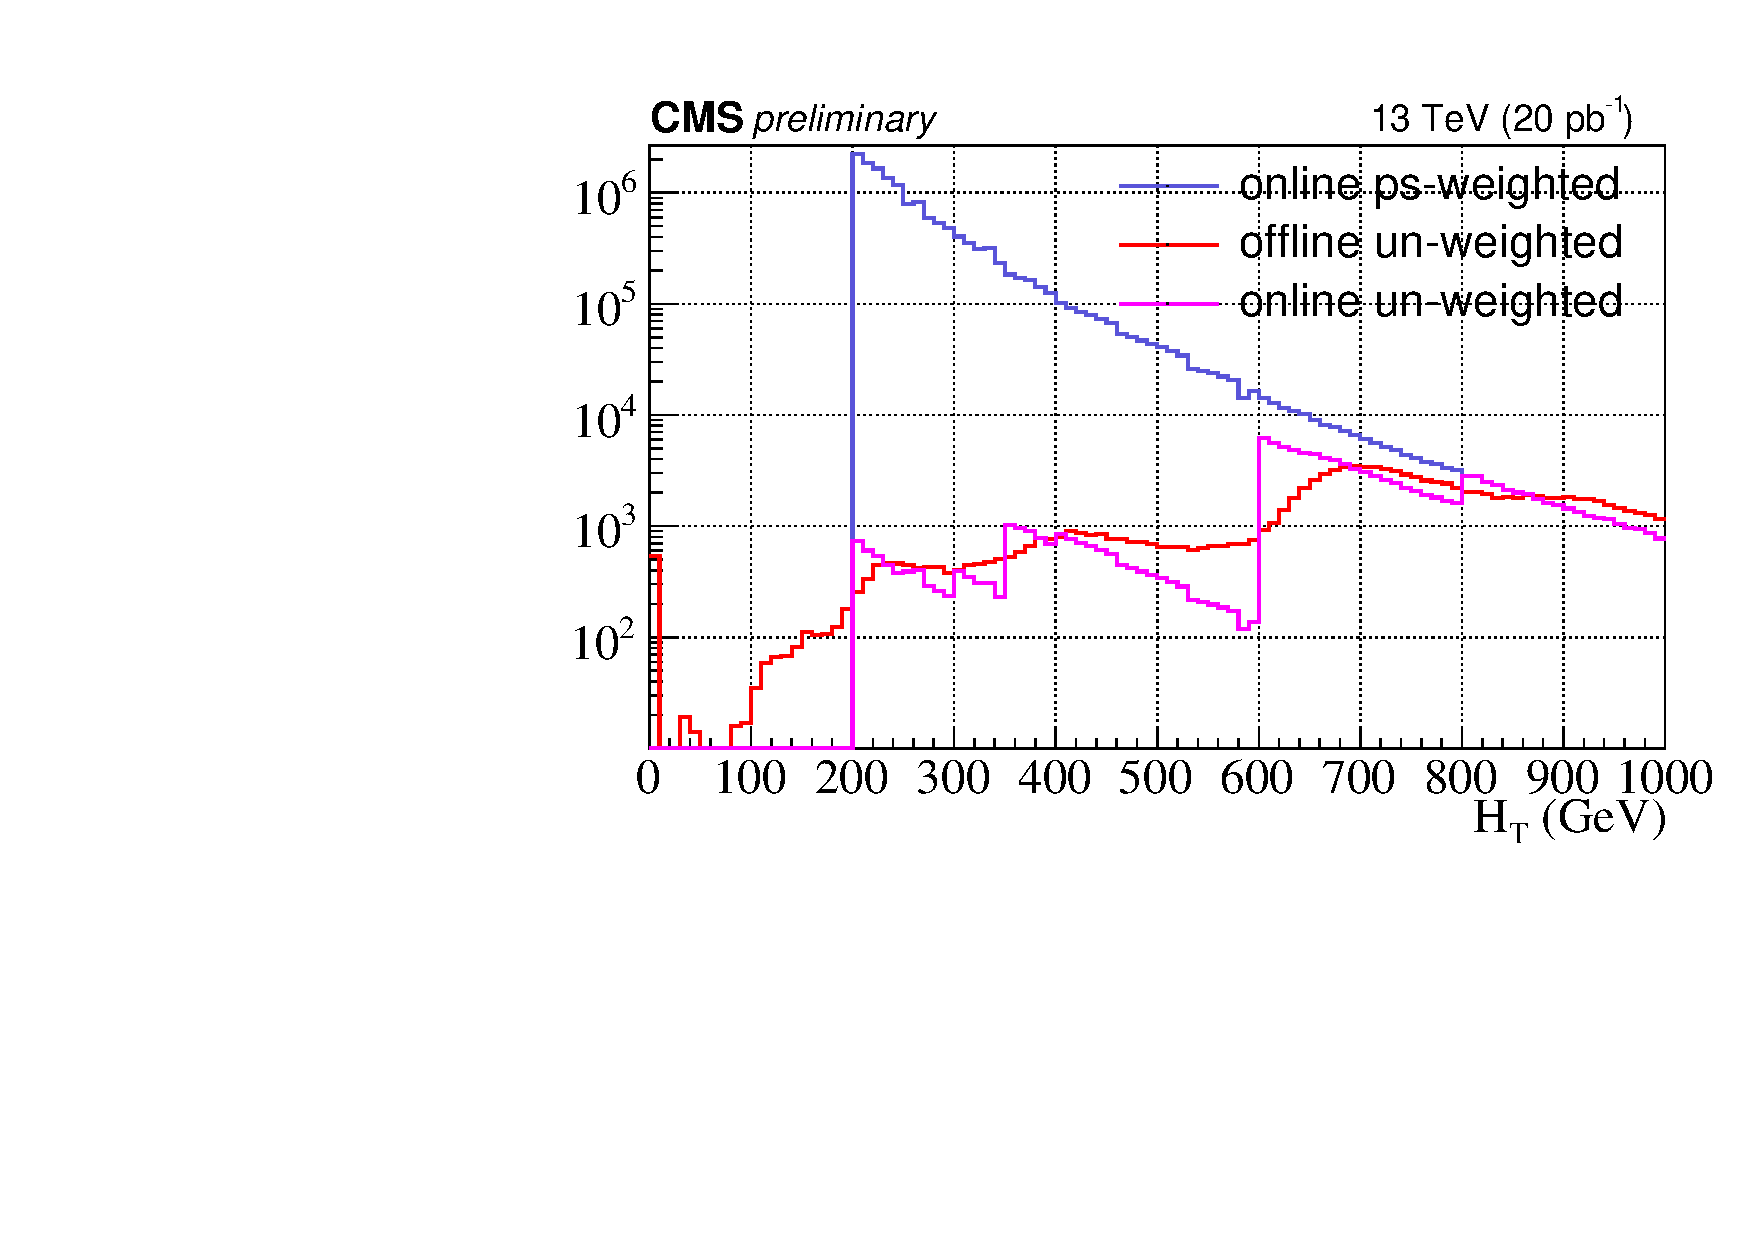
\includegraphics[width=0.6\linewidth]{figures/SusySearches/Ra2b2016/PrescaleWeightsHT2.pdf}
\caption{The distribution of the $\Ht$ in the $\Ht$ control sample for the unweighted offline $\Ht$ (red), the unweighted online $\Ht$ (pink), and the online $\Ht$ weighted by the pre-scale values.}
\label{fig:PrescaleWeights}
\end{figure}
The online pre-scale weighted $\Ht$ is smooth, as expected. The jet $\pt$ likelihoods are modified by jet resolution scale factors, derived by the jet/$\met$ POG \cite{jetmet2} to ensure the compatibility of the smearing with the true jet resolution. Rebalanced events are smeared a number of times proportional to the event's pre-scale value, which serves to apply the pre-scale weight, and ensures that all prediction events have equal weight.

\subsection{Uncertainties in the prediction}
Uncertainties in the prediction include the direct statistical uncertainty in the weighted number of counts, statistical uncertainty associated with the $\Ht$ control sample, uncertainty in the jet energy resolution, uncertainty in the parton-level $\mht$ prior density, and uncertainty corresponding to any non-closure. 

The statistical uncertainty in the prediction is the poisson uncertainty in the weighted number of counts in each bin. This uncertainty can, in principle, but reduced to arbitrarily small values by increasing the number of smearing trials. Given independent search regions, statistical uncertainties are uncorrelated across bins. 

The statistical uncertainty in the control sample is evaluated by making the prediction once using the entire data set, and once having randomly discarded half the control sample events. Scaling the half-discarded prediction up by a factor of two and taking the discrepancy with the original prediction yields a bin-by-bin systematic uncertainty. Uncertainties are once again uncorrelated across all bins.

The uncertainty in the jet energy resolution is evaluated by taking the difference between the nominal prediction and the prediction obtained by modifying the jet $\pt$ likelihoods according to the jet energy resolution uncertainties provided by  \cite{jetmet2}. Rather than evaluating the bin-by-bin discrepancy, the discrepancy in the inclusive $\mht$ distribution integrated over the bounds of each signal region between the nominal and modified predictions is taken as a percent uncertainty. This methods ensures that statistical uncertainties are not duplicated based on the limited statistics of the control sample. Uncertainties are taken to be fully correlated across all bins.

Uncertainty in the $\mht$ prior is evaluated in an analogous way as the previous uncertainty, except the difference in predictions is that between the nominal prediction and the prediction made with a modified $\mht$ prior density. The modified prior density is obtained by reweighting the nominal $\mht$ prior by the ratio of the real reconstructed $\mht$ to the simulated reconstructed $\mht$ between the values of $\mht=0$ and 200 GeV in a QCD-enriched kinematic region. The weights take values between 0.6 and 1.0, with negligible uncertainties. Uncertainties are treated as correlated across bins.

An uncertainty of 50\% is assigned to predicted counts in search bins with greater than 2 b-tags to accommodate the non-closure in simulation. In the future, this uncertainty may be eliminated by modifying the binning of the prior template as prescribe in the previous section. Non-closure uncertainties are treated as uncorrelated across bins. 

The values of the uncertainties, along with the bin-by-bin prediction, for the multi-jet$+$$\mht$ SUSY search are given in Section \ref{sec:2015results}.

